\documentclass[a4paper,11pt]{report}

\usepackage[utf8]{inputenc}
\usepackage[T1]{fontenc}
\usepackage[spanish,es-noshorthands]{babel}
\usepackage{lmodern}
\usepackage[a4paper]{geometry}
\geometry{top=2.5cm, bottom=2.5cm, left=2.2cm, right=2.2cm}

\usepackage{amsmath}
\usepackage{amssymb}
\usepackage{graphicx}
\usepackage{booktabs}
\usepackage{float}
\usepackage{caption}
\usepackage{subcaption}
\usepackage{xcolor}
\usepackage{listings}
\usepackage{enumitem}
\usepackage{tikz}
\usetikzlibrary{positioning, arrows.meta, calc}
\usepackage[hidelinks]{hyperref}

\renewcommand{\thesection}{\arabic{section}}
\setcounter{secnumdepth}{3}

% ---- Estilo de listados de codigo (Python) ----
\definecolor{codegray}{gray}{0.95}
\definecolor{codegreen}{rgb}{0.0,0.5,0.0}
\definecolor{codeblue}{rgb}{0.1,0.1,0.7}
\lstdefinestyle{py}{
  language=Python,
  backgroundcolor=\color{codegray},
  basicstyle=\ttfamily\scriptsize,
  keywordstyle=\color{codeblue}\bfseries,
  commentstyle=\color{codegreen}\itshape,
  stringstyle=\color{purple},
  numbers=left, numberstyle=\tiny\color{gray}, numbersep=6pt,
  showstringspaces=false, breaklines=true, frame=single, tabsize=4,
  captionpos=b
}
\lstset{style=py}

\title{\textbf{Control Adaptativo por Self-Tuning Regulator (STR) \\ del Péndulo Invertido en Tiempo Discreto} \\[0.4em]
\large Memoria Técnica}
\author{Lucas Gaggino \\ \small Facultad de Ingeniería - UBA \\ \small 86.20 Control Adaptativo}
\date{\today}

\begin{document}

\maketitle
\tableofcontents
\newpage

% ==================================================================
\section{Introducción}
% ==================================================================

Este trabajo implementa y valida un controlador adaptativo del tipo
\emph{Self-Tuning Regulator} (STR) para estabilizar el péndulo invertido en su
posición vertical (equilibrio inestable). El objetivo del trabajo práctico es:

\begin{enumerate}[nosep]
  \item Implementar un controlador para la planta.
  \item Evaluar su comportamiento por colocación de polos.
  \item Implementar un mecanismo de autoajuste.
  \item Validar el funcionamiento ante distintas condiciones.
\end{enumerate}

A diferencia de la implementación previa ---que estimaba un modelo por RLS, lo
convertía a tiempo continuo mediante la aproximación bilineal (Tustin) y recién
allí calculaba las ganancias PID por colocación de polos--- en esta memoria
\textbf{todo el diseño del regulador se realiza enteramente en tiempo discreto}.
No se utiliza ninguna transformación $s \leftrightarrow z$ ni librerías de
tiempo continuo: la planta se describe por su modelo ARX discreto y el
controlador se obtiene resolviendo la ecuación Diofantina en el operador
retardo $q^{-1}$, siguiendo el método STR presentado en la teoría de la materia
(\texttt{ICA\_STR.pdf}).

La estructura elegida es un \textbf{STR adaptativo indirecto}: en línea se
estiman los polinomios $A(q)$ y $B(q)$ de la planta por mínimos cuadrados
recursivos (RLS) y, por \emph{certainty equivalence}, se rediseña el regulador
resolviendo la identidad de Bézout $A R + B S = A_{lc}$.

% ==================================================================
\section{Marco Teórico: el Self-Tuning Regulator}
% ==================================================================

El material teórico de esta sección se basa en \texttt{ICA\_STR.pdf}.

\subsection{Control adaptativo y self-tuning}

Un controlador \emph{self-tuning} converge al que se hubiese hallado con las
técnicas habituales si la planta fuera conocida. Se supone conocida la
\emph{estructura} del modelo; los \emph{parámetros} son desconocidos y se
estiman on-line. Existen dos variantes:

\begin{itemize}[nosep]
  \item \textbf{Indirecto (explícito):} se estiman $A(q)$, $B(q)$ y luego se
  diseña el controlador (\emph{certainty equivalence}).
  \item \textbf{Directo (implícito):} se reparametriza el problema y se estiman
  directamente los parámetros del controlador.
\end{itemize}

En este trabajo se usa la variante \textbf{indirecta}.

\subsection{Modelo de la planta y ley de control RST}

Se considera un sistema SISO lineal expresado en el operador retardo, con una
perturbación de carga $v_k$ a la entrada:
\begin{equation}
  A(q)\, y_k = B(q)\,(u_k + v_k),
\end{equation}
con $A(q)$ mónico. La ley de control general de dos grados de libertad (RST) es:
\begin{equation}
  \boxed{\,R(q)\, u_k = T(q)\, r_k - S(q)\, y_k\,}
  \label{eq:rst}
\end{equation}
donde $S/R$ es la realimentación (\emph{feedback}) y $T/R$ el prealimentador
(\emph{feedforward}). La salida en lazo cerrado resulta:
\begin{equation}
  y_k = \frac{B\,T}{A R + B S}\, r_k + \frac{B\,R}{A R + B S}\, v_k .
  \label{eq:lc}
\end{equation}

\subsection{Diseño por colocación de polos y ecuación Diofantina}

Se impone el polinomio característico deseado de lazo cerrado $A_{lc}(q)$
mediante la \emph{identidad de Bézout} (ecuación Diofantina):
\begin{equation}
  A(q)\,R(q) + B(q)\,S(q) = A_{lc}(q).
  \label{eq:diof}
\end{equation}
Esta ecuación tiene solución si $A$ y $B$ no comparten factores. Se resuelve
algebraicamente armando la \textbf{matriz de Sylvester} (concatenación de
matrices de Toeplitz de $A$ y $B$). El \emph{controlador de mínimo orden}
cumple $\deg(R) = \deg(S)$ y $\deg(S) = \deg(A) - 1$, con
$\deg(A_{lc}) = 2\deg(A) - 1$.

\subsection{Rechazo de perturbaciones}

Del numerador de la perturbación en \eqref{eq:lc}, $B\,R$, se desprenden las
reglas de diseño:
\begin{itemize}[nosep]
  \item \textbf{Perturbación de carga escalón en $v$:} $B$ o $R$ deben tener una
  raíz en $z=1$. La clave está en diseñar $R$ con el factor $(1-q^{-1})$
  (acción integral).
  \item \textbf{Ruido de medición $e$:} para no amplificar alta frecuencia se
  puede forzar un término $z+1$ en $S$ (aquí no es necesario porque el estimador
  RLS ya filtra el ruido).
\end{itemize}

\subsection{Estimación recursiva (RLS con olvido)}

Para un modelo ARX, con vector de parámetros
$\theta = [a_1,\dots,a_n, b_1,\dots,b_m]^\top$ y regresor $\varphi(k)$, el RLS
con factor de olvido $\lambda \in (0,1]$ es:
\begin{align}
  \epsilon(k) &= y(k) - \varphi^\top(k)\,\hat\theta(k-1), \\
  K(k) &= \frac{P(k-1)\varphi(k)}{\lambda + \varphi^\top(k)P(k-1)\varphi(k)}, \\
  \hat\theta(k) &= \hat\theta(k-1) + K(k)\,\epsilon(k), \\
  P(k) &= \tfrac{1}{\lambda}\big(I - K(k)\varphi^\top(k)\big)P(k-1).
\end{align}
$\lambda \to 1$ permite seguir parámetros lentamente variables; valores menores
olvidan más rápido a costa de mayor sensibilidad al ruido.

\subsection{Algoritmo indirecto}

\begin{enumerate}[nosep]
  \item En cada $k$, recolectar $\varphi(k)$ e $y(k)$.
  \item Actualizar RLS $\Rightarrow \hat A(q), \hat B(q)$.
  \item Resolver la Diofantina \eqref{eq:diof} $\Rightarrow R, S, T$.
  \item Calcular la acción de control con \eqref{eq:rst}.
  \item Aplicar $u(k)$ y repetir.
\end{enumerate}
No es necesario recalcular el controlador en cada paso: puede hacerse cada $N$
pasos. Es crítico garantizar la \emph{persistencia de excitación}.

% ==================================================================
\section{Sistema: el Péndulo Invertido}
% ==================================================================

\subsection{Modelo no lineal}

La planta ``real'' que se controla en la simulación es el modelo no lineal del
carro-péndulo, con estado $[x, \dot x, \theta, \dot\theta]$:
\begin{equation}
  \ddot\theta = \frac{g\sin\theta - \cos\theta \cdot \dfrac{F + m l \dot\theta^2 \sin\theta}{M+m}}
  {l\left(\tfrac{4}{3} - \dfrac{m\cos^2\theta}{M+m}\right)},
\end{equation}
con $M = 1{,}0$~kg, $m = 0{,}1$~kg, $l = 0{,}5$~m, $g = 9{,}81$~m/s$^2$. Se
integra con Runge-Kutta manteniendo la acción de control constante en cada
período (ZOH).

\subsection{Linealización}

Alrededor del equilibrio inestable ($\theta = 0$):
\begin{equation}
  \ddot\theta = A_\theta\,\theta + B_\theta\,F, \qquad
  A_\theta = \frac{3g(M+m)}{l(4M+m)} = 15{,}79, \qquad
  B_\theta = \frac{-3}{l(4M+m)} = -1{,}4634 .
\end{equation}
El signo $B_\theta < 0$ es físicamente correcto: un empuje $F>0$ sobre el carro
reduce $\theta$. Este signo es esencial: usar el signo opuesto produce
realimentación positiva y el lazo diverge.

\subsection{Discretización ZOH analítica y modelo ARX}

En lugar de usar librerías de tiempo continuo, se discretiza analíticamente.
Para $G(s) = B_\theta/(s^2 - w^2)$ con $w = \sqrt{A_\theta}$, el mantenedor de
orden cero da:
\begin{equation}
  A(z) = z^2 - 2\cosh(w T_s)\, z + 1, \qquad
  B(z) = \frac{B_\theta(\cosh(w T_s) - 1)}{A_\theta}\,(z + 1),
\end{equation}
con $T_s = 0{,}02$~s. Numéricamente, el modelo ARX nominal es:
\begin{equation}
  A(q) = 1 - 2{,}0063\,q^{-1} + 1{,}0\,q^{-2}, \qquad
  B(q) = -2{,}93\!\times\!10^{-4}\,(q^{-1} + q^{-2}).
\end{equation}

\paragraph{Observaciones de diseño.} La planta discreta tiene un polo en
$z \approx 1{,}083$ (\emph{fuera} del círculo unitario, inestable) y otro en
$z \approx 0{,}924$. El cero está en $z \approx -1$ (sobre el círculo unitario):
es \textbf{no de fase mínima}, por lo que \textbf{no se lo cancela} (cancelarlo
generaría oscilaciones de alta amplitud, \emph{ringing}). Este modelo nominal se
usa solo como \emph{prior} de arranque del STR; los parámetros reales se estiman
on-line.

% ==================================================================
\section{Diseño del Regulador STR (paso a paso)}
% ==================================================================

\subsection{Estructura elegida}

STR indirecto, por colocación de polos, \textbf{sin cancelación de ceros} y
\textbf{con integrador}. Para incorporar la acción integral se diseña sobre
\begin{equation}
  \bar A(q) = A(q)\,(1 - q^{-1}),
\end{equation}
de grado 3, y luego $R = (1-q^{-1})\,\bar R$.

\subsection{Elección de los polos de lazo cerrado}

Se reutiliza la especificación del diseño previo ($s = -3, -3, -10$),
mapeada a discreto con $z = e^{s T_s}$:
\begin{equation}
  \{-3,-3,-10\} \;\to\; \{0{,}9418,\ 0{,}9418,\ 0{,}8187\}.
\end{equation}
La Diofantina con integrador requiere $\deg(A_{lc}) = 5$, por lo que se agregan
dos polos auxiliares rápidos en $z = 0{,}2$ (bien amortiguados, cerca del
origen) para completar el grado sin alterar la dinámica dominante:
\begin{equation}
  A_{lc}(z) = (z-0{,}9418)^2 (z-0{,}8187)(z-0{,}2)^2 .
\end{equation}

\subsection{Grados y causalidad}

Con $\deg(\bar A) = 3$ y $\deg(B) = 2$, el controlador de mínimo orden tiene
$\deg(\bar R) = 2$ y $\deg(S) = 2$. El regulador final:
\begin{equation}
  R(q) = (1-q^{-1})\,\bar R(q) \ (\text{grado }3), \qquad
  S(q) = s_0 + s_1 q^{-1} + s_2 q^{-2}.
\end{equation}

\subsection{Resolución de la ecuación Diofantina (matriz de Sylvester)}

Se resuelve $\bar A(q)\,\bar R(q) + B(q)\,S(q) = A_{lc}(q)$ con
$\bar A = [1, \bar a_1, \bar a_2, \bar a_3]$, $B = [0, b_1, b_2]$,
$\bar R = [1, r_1, r_2]$ y $S = [s_0, s_1, s_2]$. Igualando coeficientes de
$q^{-1}$ a $q^{-5}$ se obtiene el sistema lineal (matriz de Sylvester):
\begin{equation}
\begin{bmatrix}
1 & 0 & b_1 & 0 & 0 \\
\bar a_1 & 1 & b_2 & b_1 & 0 \\
\bar a_2 & \bar a_1 & 0 & b_2 & b_1 \\
\bar a_3 & \bar a_2 & 0 & 0 & b_2 \\
0 & \bar a_3 & 0 & 0 & 0
\end{bmatrix}
\begin{bmatrix} r_1 \\ r_2 \\ s_0 \\ s_1 \\ s_2 \end{bmatrix}
=
\begin{bmatrix}
\alpha_1 - \bar a_1 \\ \alpha_2 - \bar a_2 \\ \alpha_3 - \bar a_3 \\ \alpha_4 \\ \alpha_5
\end{bmatrix},
\end{equation}
donde $\alpha_i$ son los coeficientes de $A_{lc}$. Para el modelo nominal
($\bar A = [1, -3{,}0063,\ 3{,}0063,\ -1{,}0]$) la solución es:
\begin{equation}
  R = [\,1,\ -1{,}2033,\ 0{,}2324,\ -0{,}0290\,], \quad
  S = [\,-366{,}77,\ 697{,}19,\ -331{,}09\,].
\end{equation}
Los valores grandes de $S$ reflejan la alta ganancia necesaria para estabilizar
un sistema inestable.

\subsection{Prealimentación (ganancia estática unitaria)}

Se impone $y/r|_{q^{-1}=1} = 1$, es decir $B(1)\,T / A_{lc}(1) = 1$, de donde
\begin{equation}
  T = t_0 = \frac{A_{lc}(1)}{B(1)} = \frac{\sum_i \alpha_i}{b_1 + b_2} = -0{,}6718 .
\end{equation}
Como la referencia es $\theta = 0$, el término $T\,r$ es nulo, pero se deja
general.

\subsection{Diagrama de bloques}

\begin{figure}[H]
\centering
\begin{tikzpicture}[>=Latex, node distance=1.4cm, auto,
  block/.style={draw, rectangle, minimum height=1cm, minimum width=1.6cm, align=center},
  sum/.style={draw, circle, inner sep=0pt, minimum size=6mm}]
  \node (r) {$r_k$};
  \node[block, right=1.2cm of r] (T) {$\dfrac{T}{R}$};
  \node[sum, right=1.2cm of T] (s1) {$+$};
  \node[block, right=1.2cm of s1] (P) {$\dfrac{B}{A}$ \\ \small planta};
  \node[right=1.6cm of P] (y) {$y_k$};
  \node[block, below=1.2cm of s1] (S) {$\dfrac{S}{R}$};

  \draw[->] (r) -- (T);
  \draw[->] (T) -- (s1);
  \draw[->] (s1) -- node {$u_k$} (P);
  \draw[->] (P) -- (y);
  \draw[->] ($(P)!0.5!(y)$) |- (S);
  \draw[->] (S) -| node[pos=0.95, left] {$-$} (s1);
\end{tikzpicture}
\caption{Estructura RST de dos grados de libertad: feedforward $T/R$,
feedback $S/R$ y planta $B/A$. La ley $R u = T r - S y$ incluye el integrador
$(1-q^{-1})$ en $R$.}
\label{fig:blk}
\end{figure}

% ==================================================================
\section{Implementación}
% ==================================================================

El código está en \texttt{respuesta\_pid\_pendulo\_autotunning.py}. Se resumen
las piezas centrales.

\subsection{Estimador RLS}

\begin{lstlisting}[caption={Un paso de RLS con olvido.}]
def rls_step(theta, P, phi, y_meas, lambda_=0.995):
    y_pred = phi @ theta
    err = y_meas - y_pred
    Pphi = P @ phi
    K = Pphi / (lambda_ + phi @ Pphi)
    theta = theta + K * err
    P = (P - np.outer(K, Pphi)) / lambda_
    return theta, P, err
\end{lstlisting}

\subsection{Ecuacion Diofantina (Sylvester) y diseno RST}

\begin{lstlisting}[caption={Armado de la matriz de Sylvester y resolucion.}]
def solve_diophantine_sylvester(A_bar, B, Alc, deg_R, deg_S):
    n_rows = len(Alc)
    n_unk = deg_R + (deg_S + 1)
    M_syl = np.zeros((n_rows, n_unk))
    for i in range(1, deg_R + 1):          # columnas de r_i (A_bar desplazado)
        for k in range(len(A_bar)):
            M_syl[i + k, i - 1] += A_bar[k]
    off = deg_R
    for j in range(0, deg_S + 1):          # columnas de s_j (B desplazado)
        for k in range(len(B)):
            M_syl[j + k, off + j] += B[k]
    rhs = Alc.copy()
    for k in range(len(A_bar)):            # pasar termino monico de R a la der.
        rhs[k] -= A_bar[k]
    sol = np.linalg.solve(M_syl[1:1 + n_unk, :], rhs[1:1 + n_unk])
    return np.concatenate(([1.0], sol[:deg_R])), sol[deg_R:]
\end{lstlisting}

\begin{lstlisting}[caption={Diseno del regulador con integrador y sin cancelacion.}]
def design_rst(theta_hat, polos_lc=POLOS_LC):
    a1, a2, b1, b2 = theta_hat
    A = np.array([1.0, a1, a2])
    B = np.array([0.0, b1, b2])
    A_bar = np.convolve(A, [1.0, -1.0])    # integrador: A*(1 - q^-1)
    Alc = np.real(np.poly(polos_lc))       # A_lc deseado
    R_bar, S = solve_diophantine_sylvester(A_bar, B, Alc, deg_R=2, deg_S=2)
    R = np.convolve([1.0, -1.0], R_bar)
    t0 = np.sum(Alc) / (b1 + b2)           # ganancia estatica unitaria
    return R, S, t0
\end{lstlisting}

\subsection{Controlador RST}

\begin{lstlisting}[caption={Ley recursiva R u = T r - S y.}]
def control(self, r, y):
    yvec = np.concatenate(([y], self.y_hist))[:len(self.S)]
    s_term = float(self.S @ yvec)
    r_term = float(self.R[1:] @ self.u_hist[:len(self.R) - 1])
    u = (self.t0 * r - s_term - r_term) / self.R[0]
    # ... actualizar historiales de u e y ...
    return u
\end{lstlisting}

\subsection{Bucle adaptativo}

En cada paso: (i) RLS actualiza $\hat\theta = [a_1,a_2,b_1,b_2]$; (ii) tras un
\emph{warmup} y cada \texttt{redesign\_every} pasos se rediseña el RST; (iii) se
aplica la acción de control; (iv) se integra la ODE no lineal (ZOH). Dos
salvaguardas importantes:
\begin{itemize}[nosep]
  \item \textbf{Freno por baja excitación:} el RLS solo actualiza si
  $\lVert\varphi\rVert$ supera un umbral. Al estabilizarse el péndulo, las
  señales tienden a cero y sin este freno el estimador se degradaría (problema
  de persistencia de excitación).
  \item \textbf{Guarda de divergencia:} si $|\theta| > 90^\circ$ (el péndulo
  ``cayó'') se detiene la integración.
\end{itemize}

\begin{lstlisting}[caption={Nucleo del bucle de simulacion.}]
if k >= 2:
    phi = np.array([-y[k-1], -y[k-2], u[k-1], u[k-2]])
    if np.linalg.norm(phi) > excite_thresh:
        theta_hat, P, _ = rls_step(theta_hat, P, phi, y_measured, lambda_)

if k >= warmup_k and (k - warmup_k) % redesign_every == 0:
    R_new, S_new, t0_new = design_rst(theta_hat)   # certainty equivalence
    ctrl_rst.set_params(R_new, S_new, t0_new)

u_control = ctrl_rst.control(ref[k], y_measured)
\end{lstlisting}

% ==================================================================
\section{Resultados y Validación}
% ==================================================================

Se simularon 20~s desde la condición inicial $\theta(0) = 0{,}1$~rad con
referencia $\theta = 0$, en cuatro escenarios. En todos, el ángulo se estabiliza
(nunca supera la condición inicial) y la acción de control se mantiene acotada
($|u|_{\max} \approx 37$~N). Sin perturbaciones, la estimación RLS converge al
modelo real
$[a_1,a_2,b_1,b_2] \approx [-2{,}006,\ 1{,}0,\ -2{,}9\!\times\!10^{-4},\ -2{,}9\!\times\!10^{-4}]$.
El análisis de convergencia del regulador ante ruido y perturbaciones se detalla
en la Sección~7.

\begin{figure}[H]
\centering
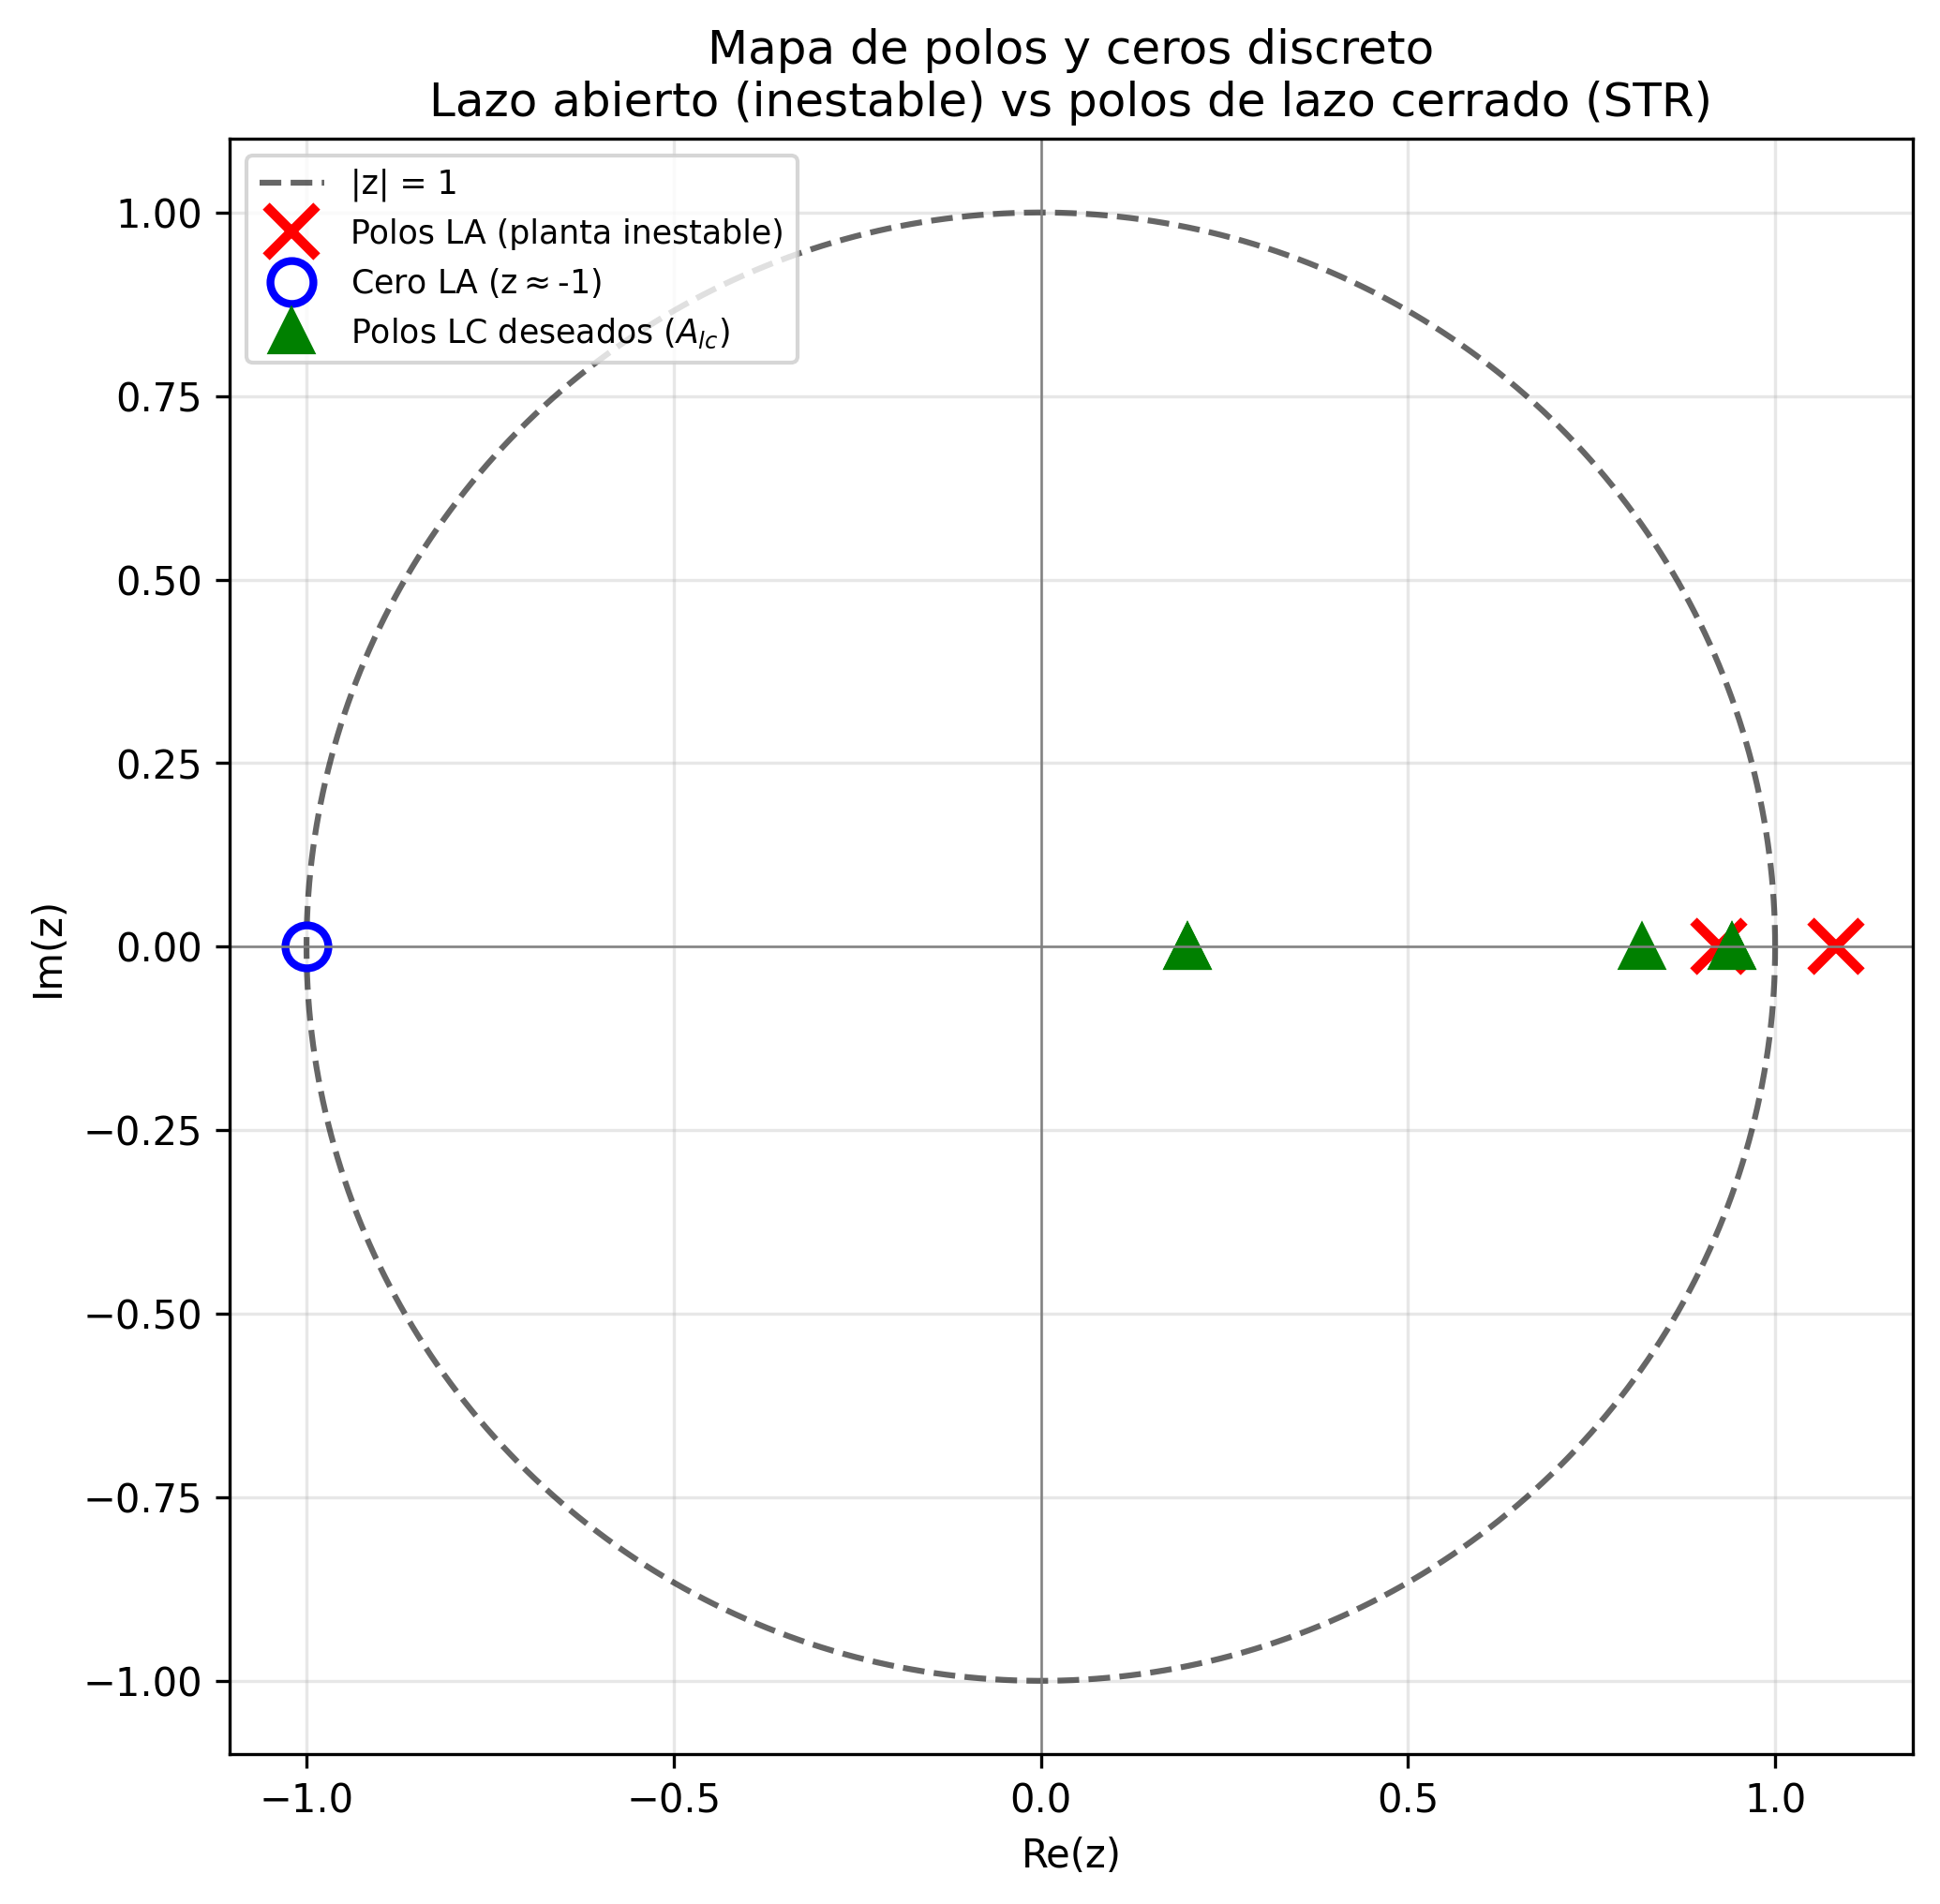
\includegraphics[width=0.85\textwidth]{presentacion_pid_pendulo/imagenes_pid_autotunning/str_polos_ceros.png}
\caption{Mapa de polos y ceros discreto. El polo de lazo abierto fuera del
círculo unitario (planta inestable) y el cero en $z\approx-1$; los polos de lazo
cerrado impuestos por el STR quedan dentro del círculo unitario.}
\label{fig:pz}
\end{figure}

\begin{figure}[H]
\centering
\begin{subfigure}{0.49\textwidth}
  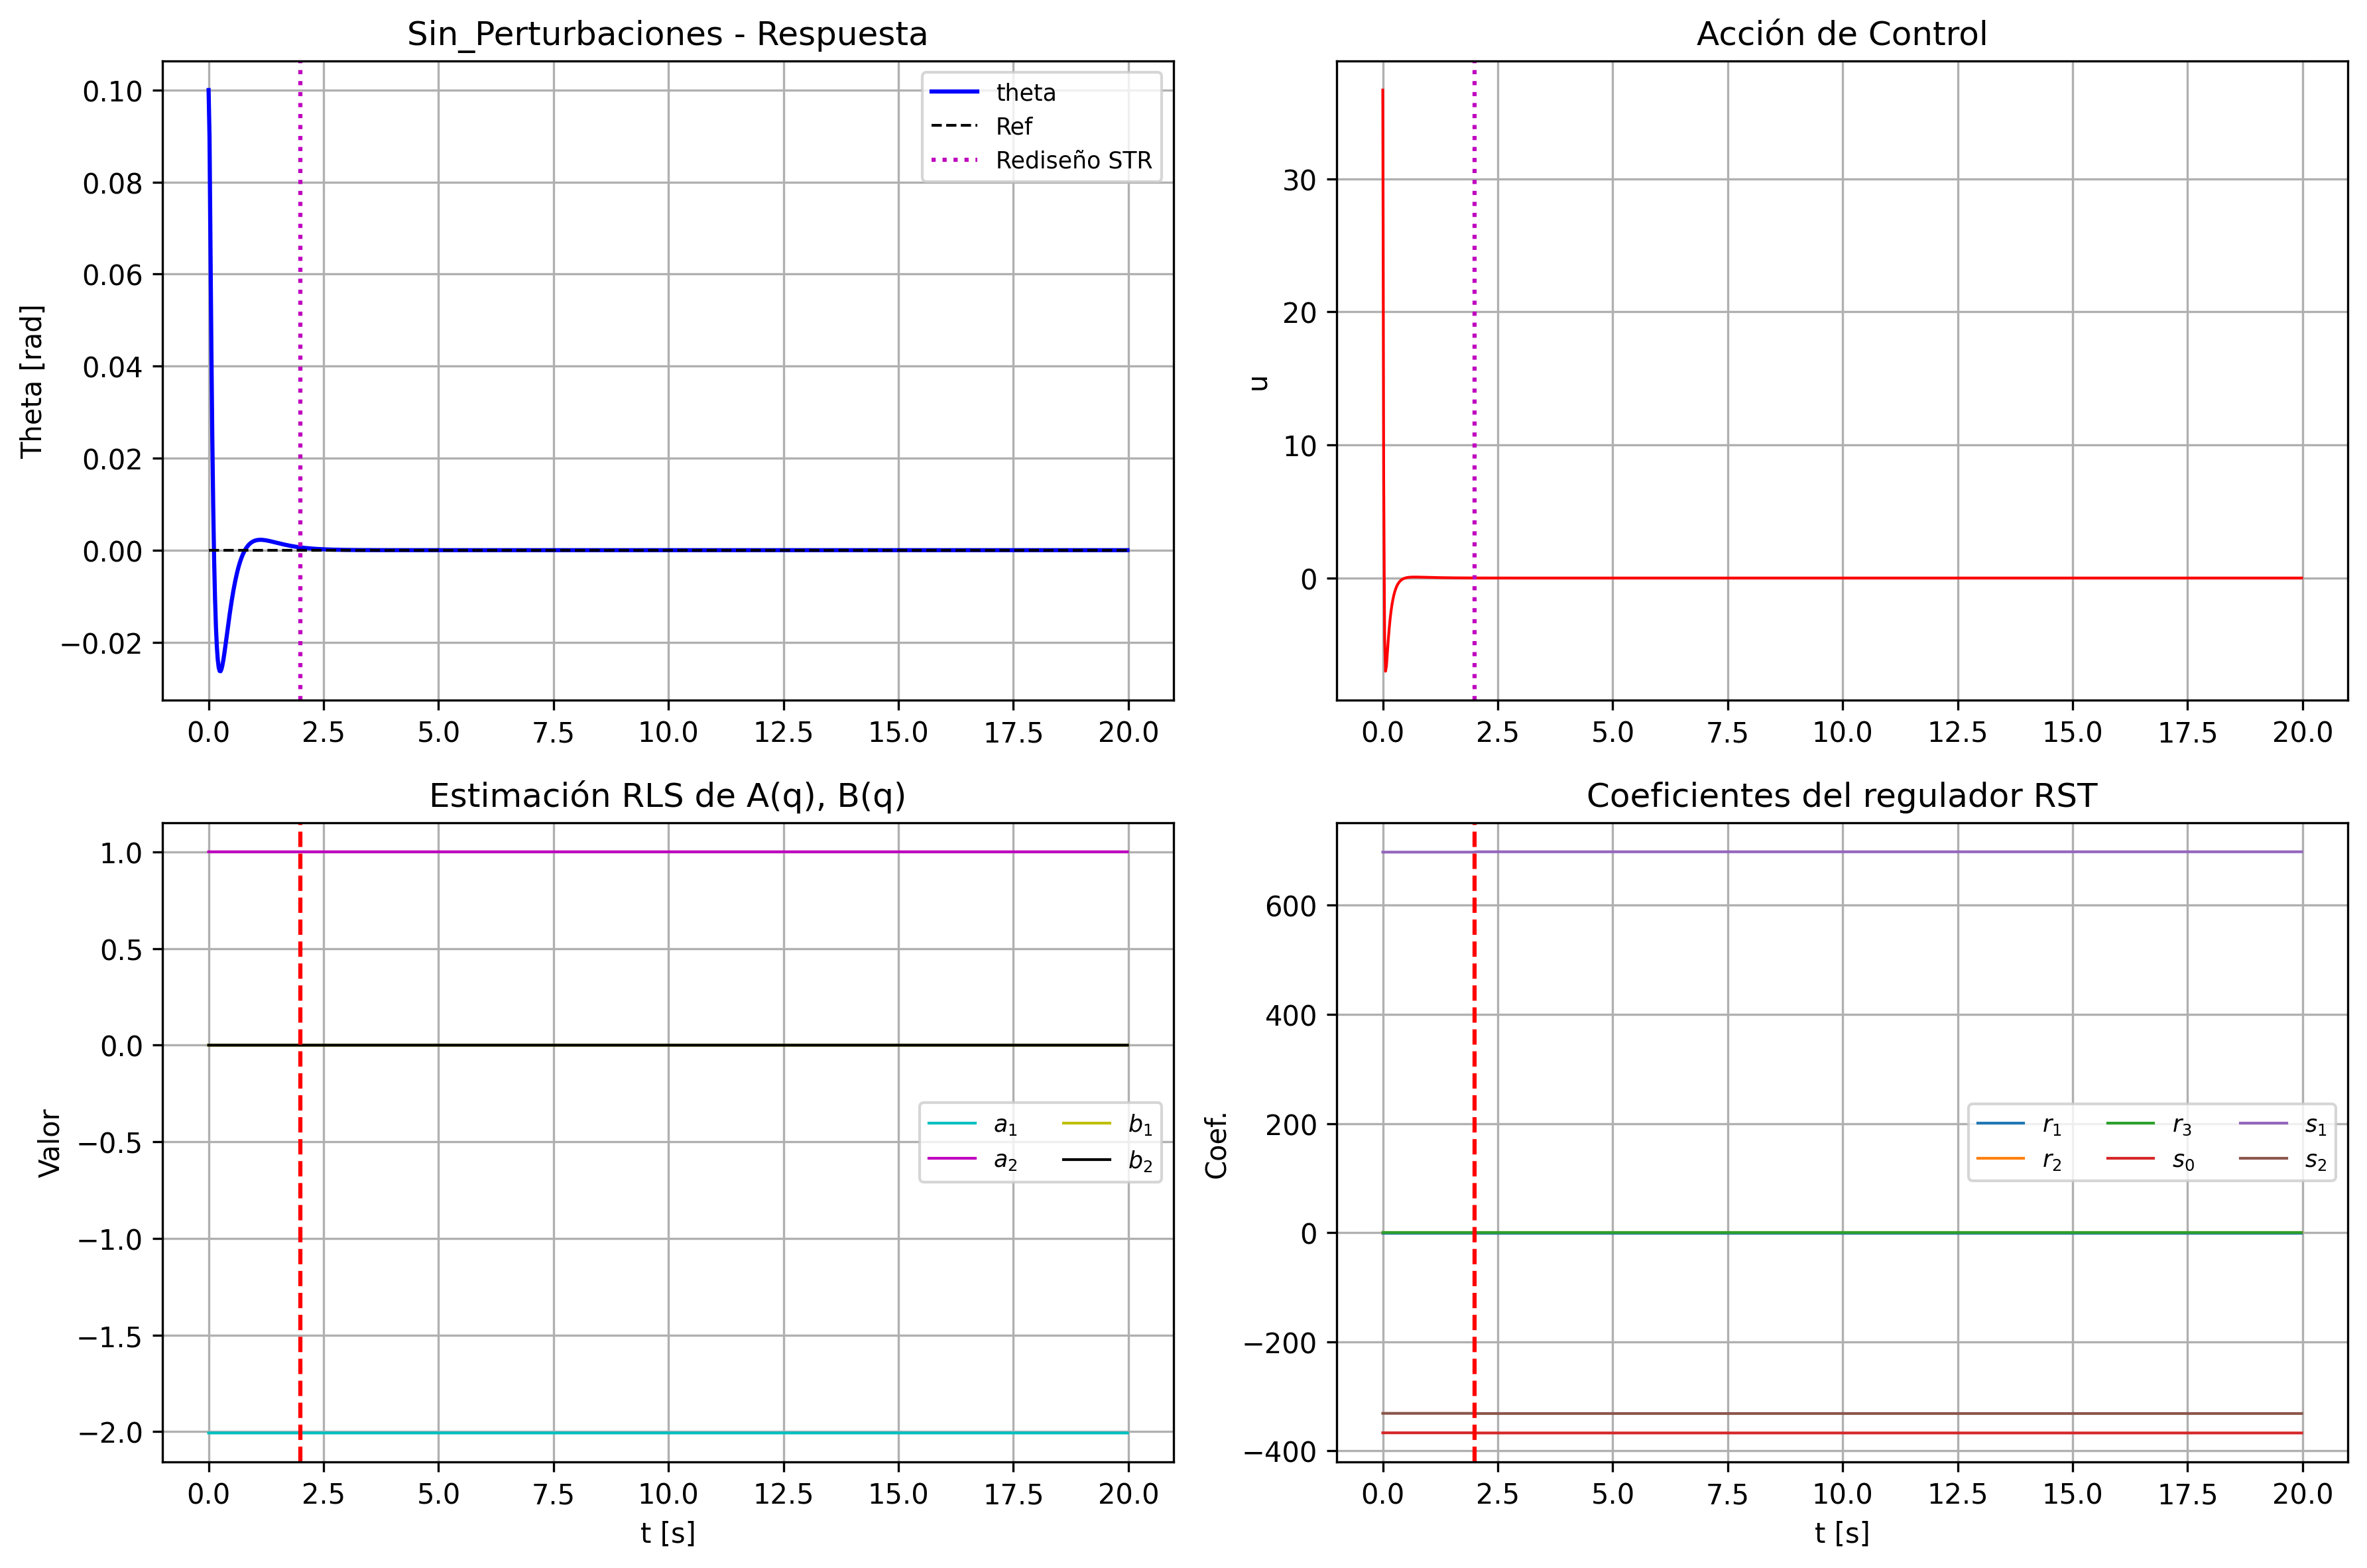
\includegraphics[width=\textwidth]{presentacion_pid_pendulo/imagenes_pid_autotunning/str_Sin_Perturbaciones.png}
  \caption{Sin perturbaciones}
\end{subfigure}
\hfill
\begin{subfigure}{0.49\textwidth}
  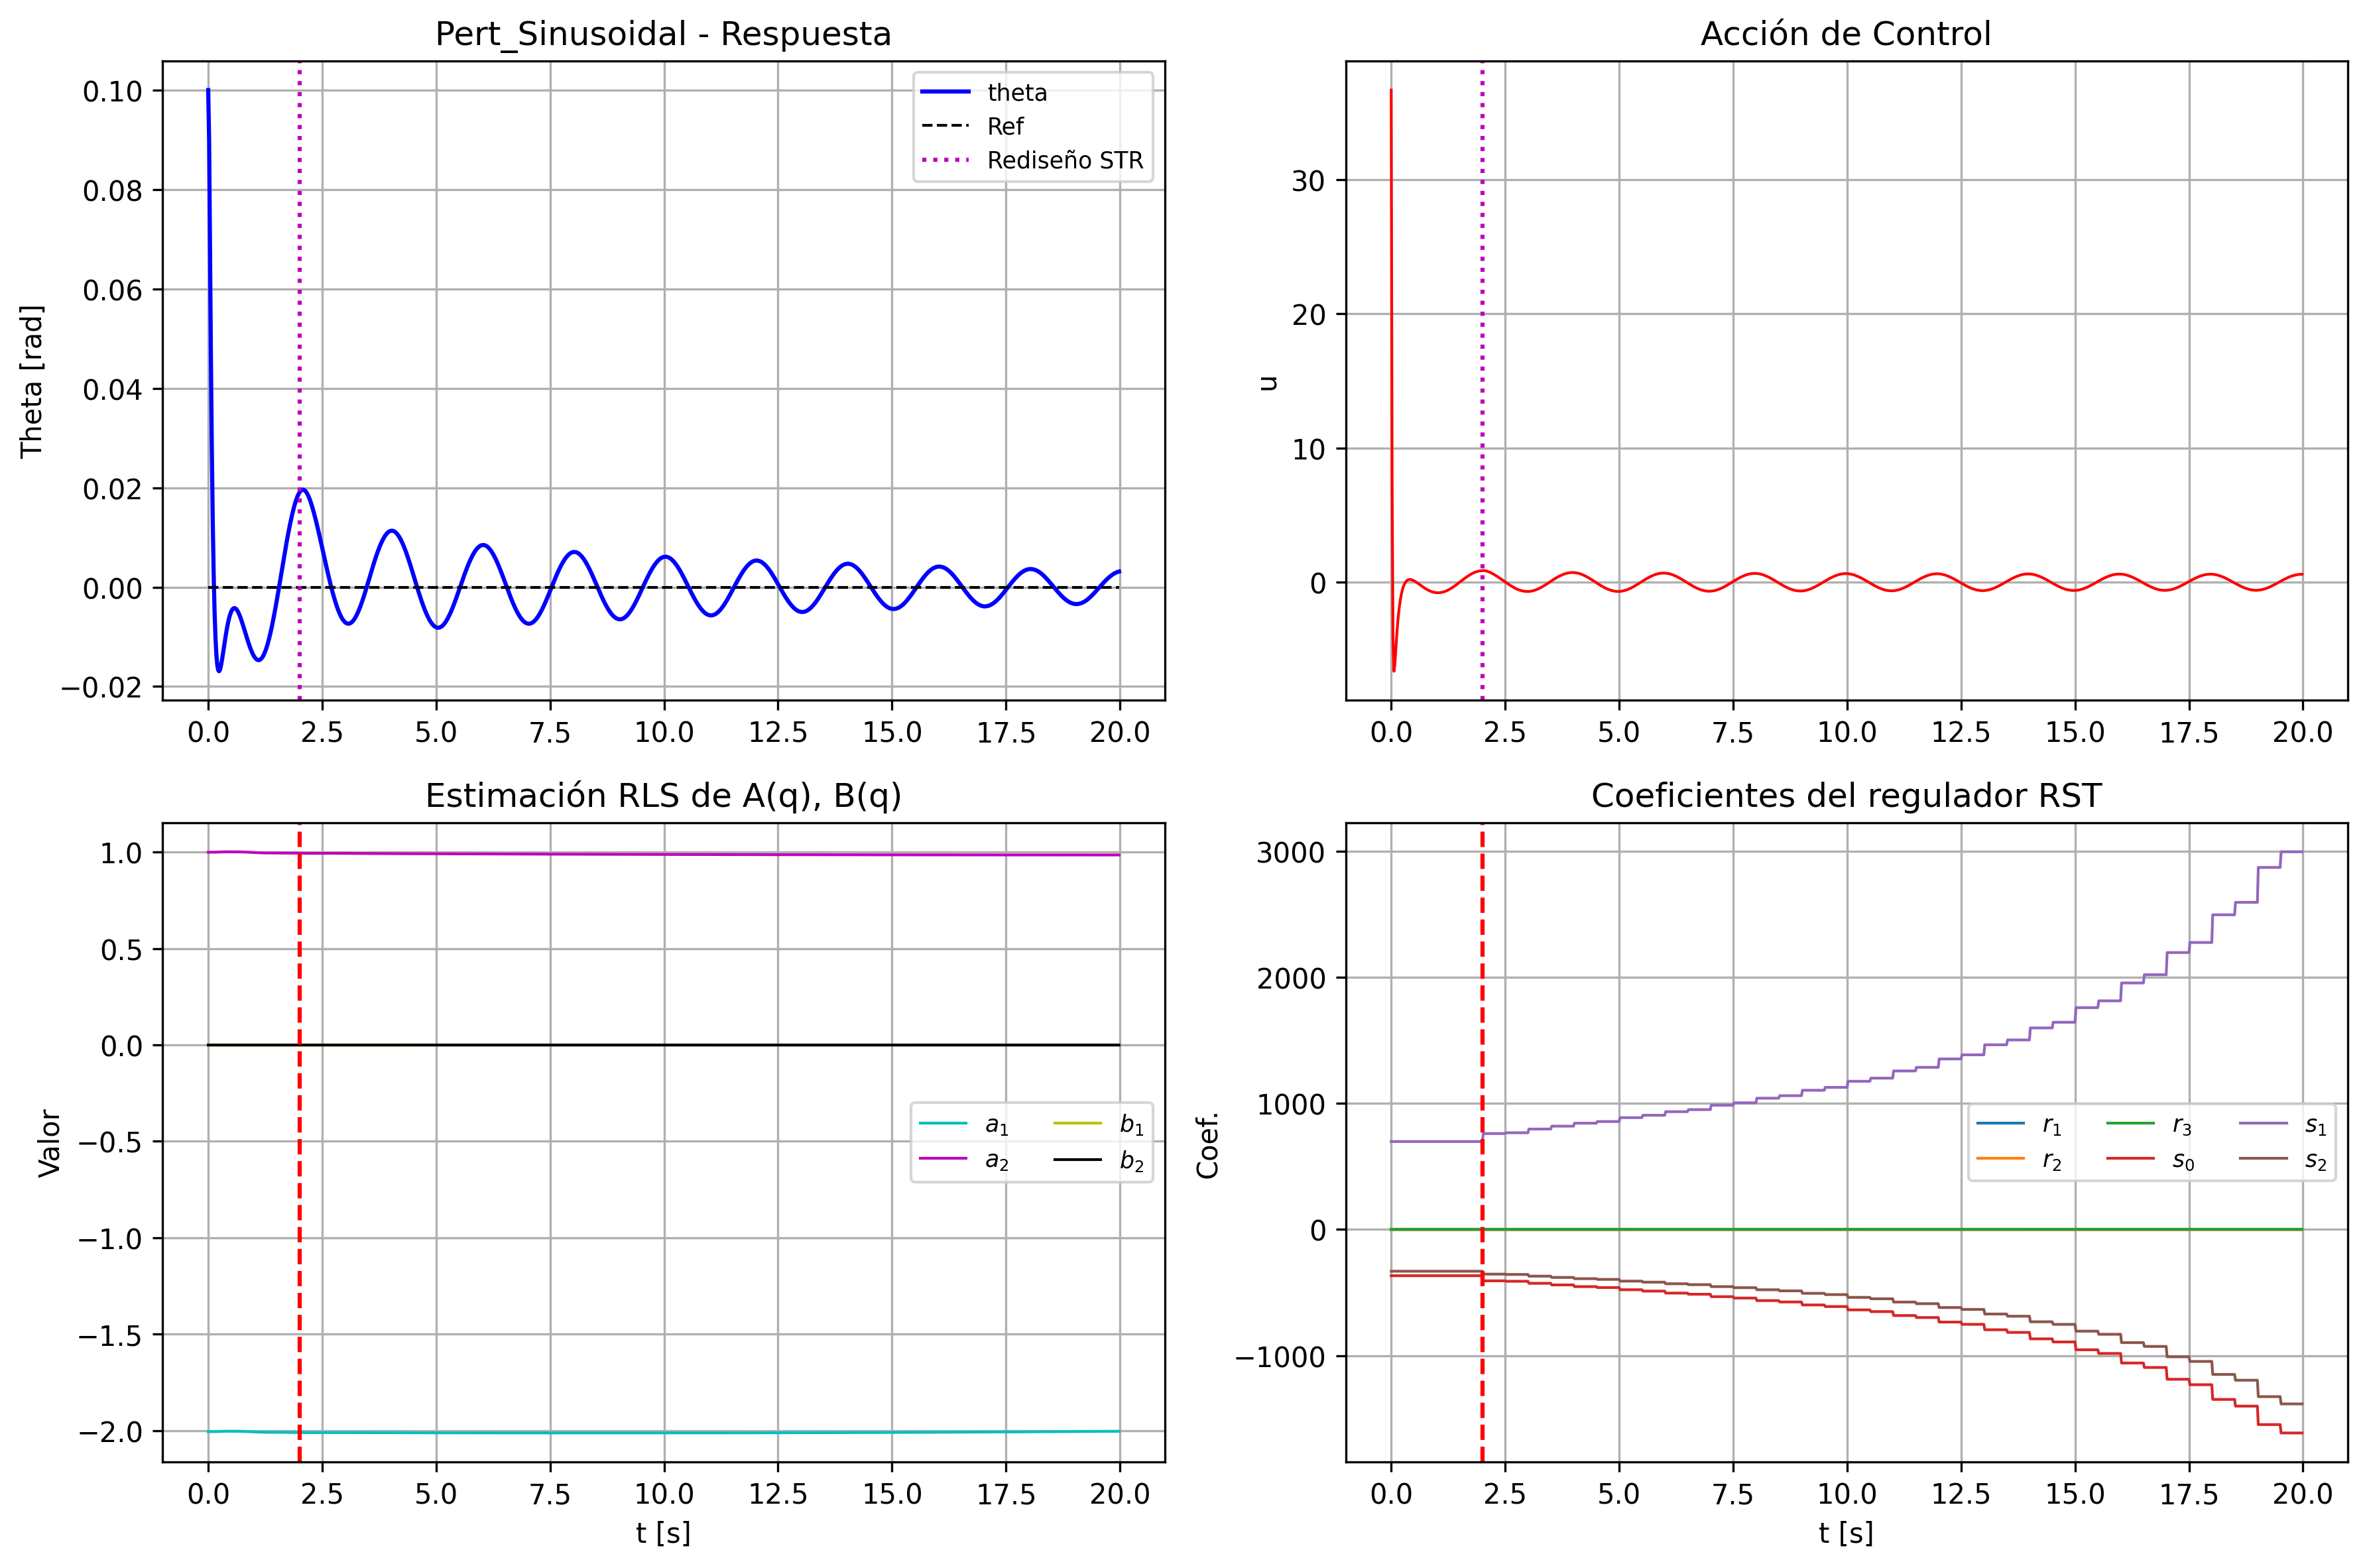
\includegraphics[width=\textwidth]{presentacion_pid_pendulo/imagenes_pid_autotunning/str_Pert_Sinusoidal.png}
  \caption{Perturbación sinusoidal}
\end{subfigure}
\\[0.5em]
\begin{subfigure}{0.49\textwidth}
  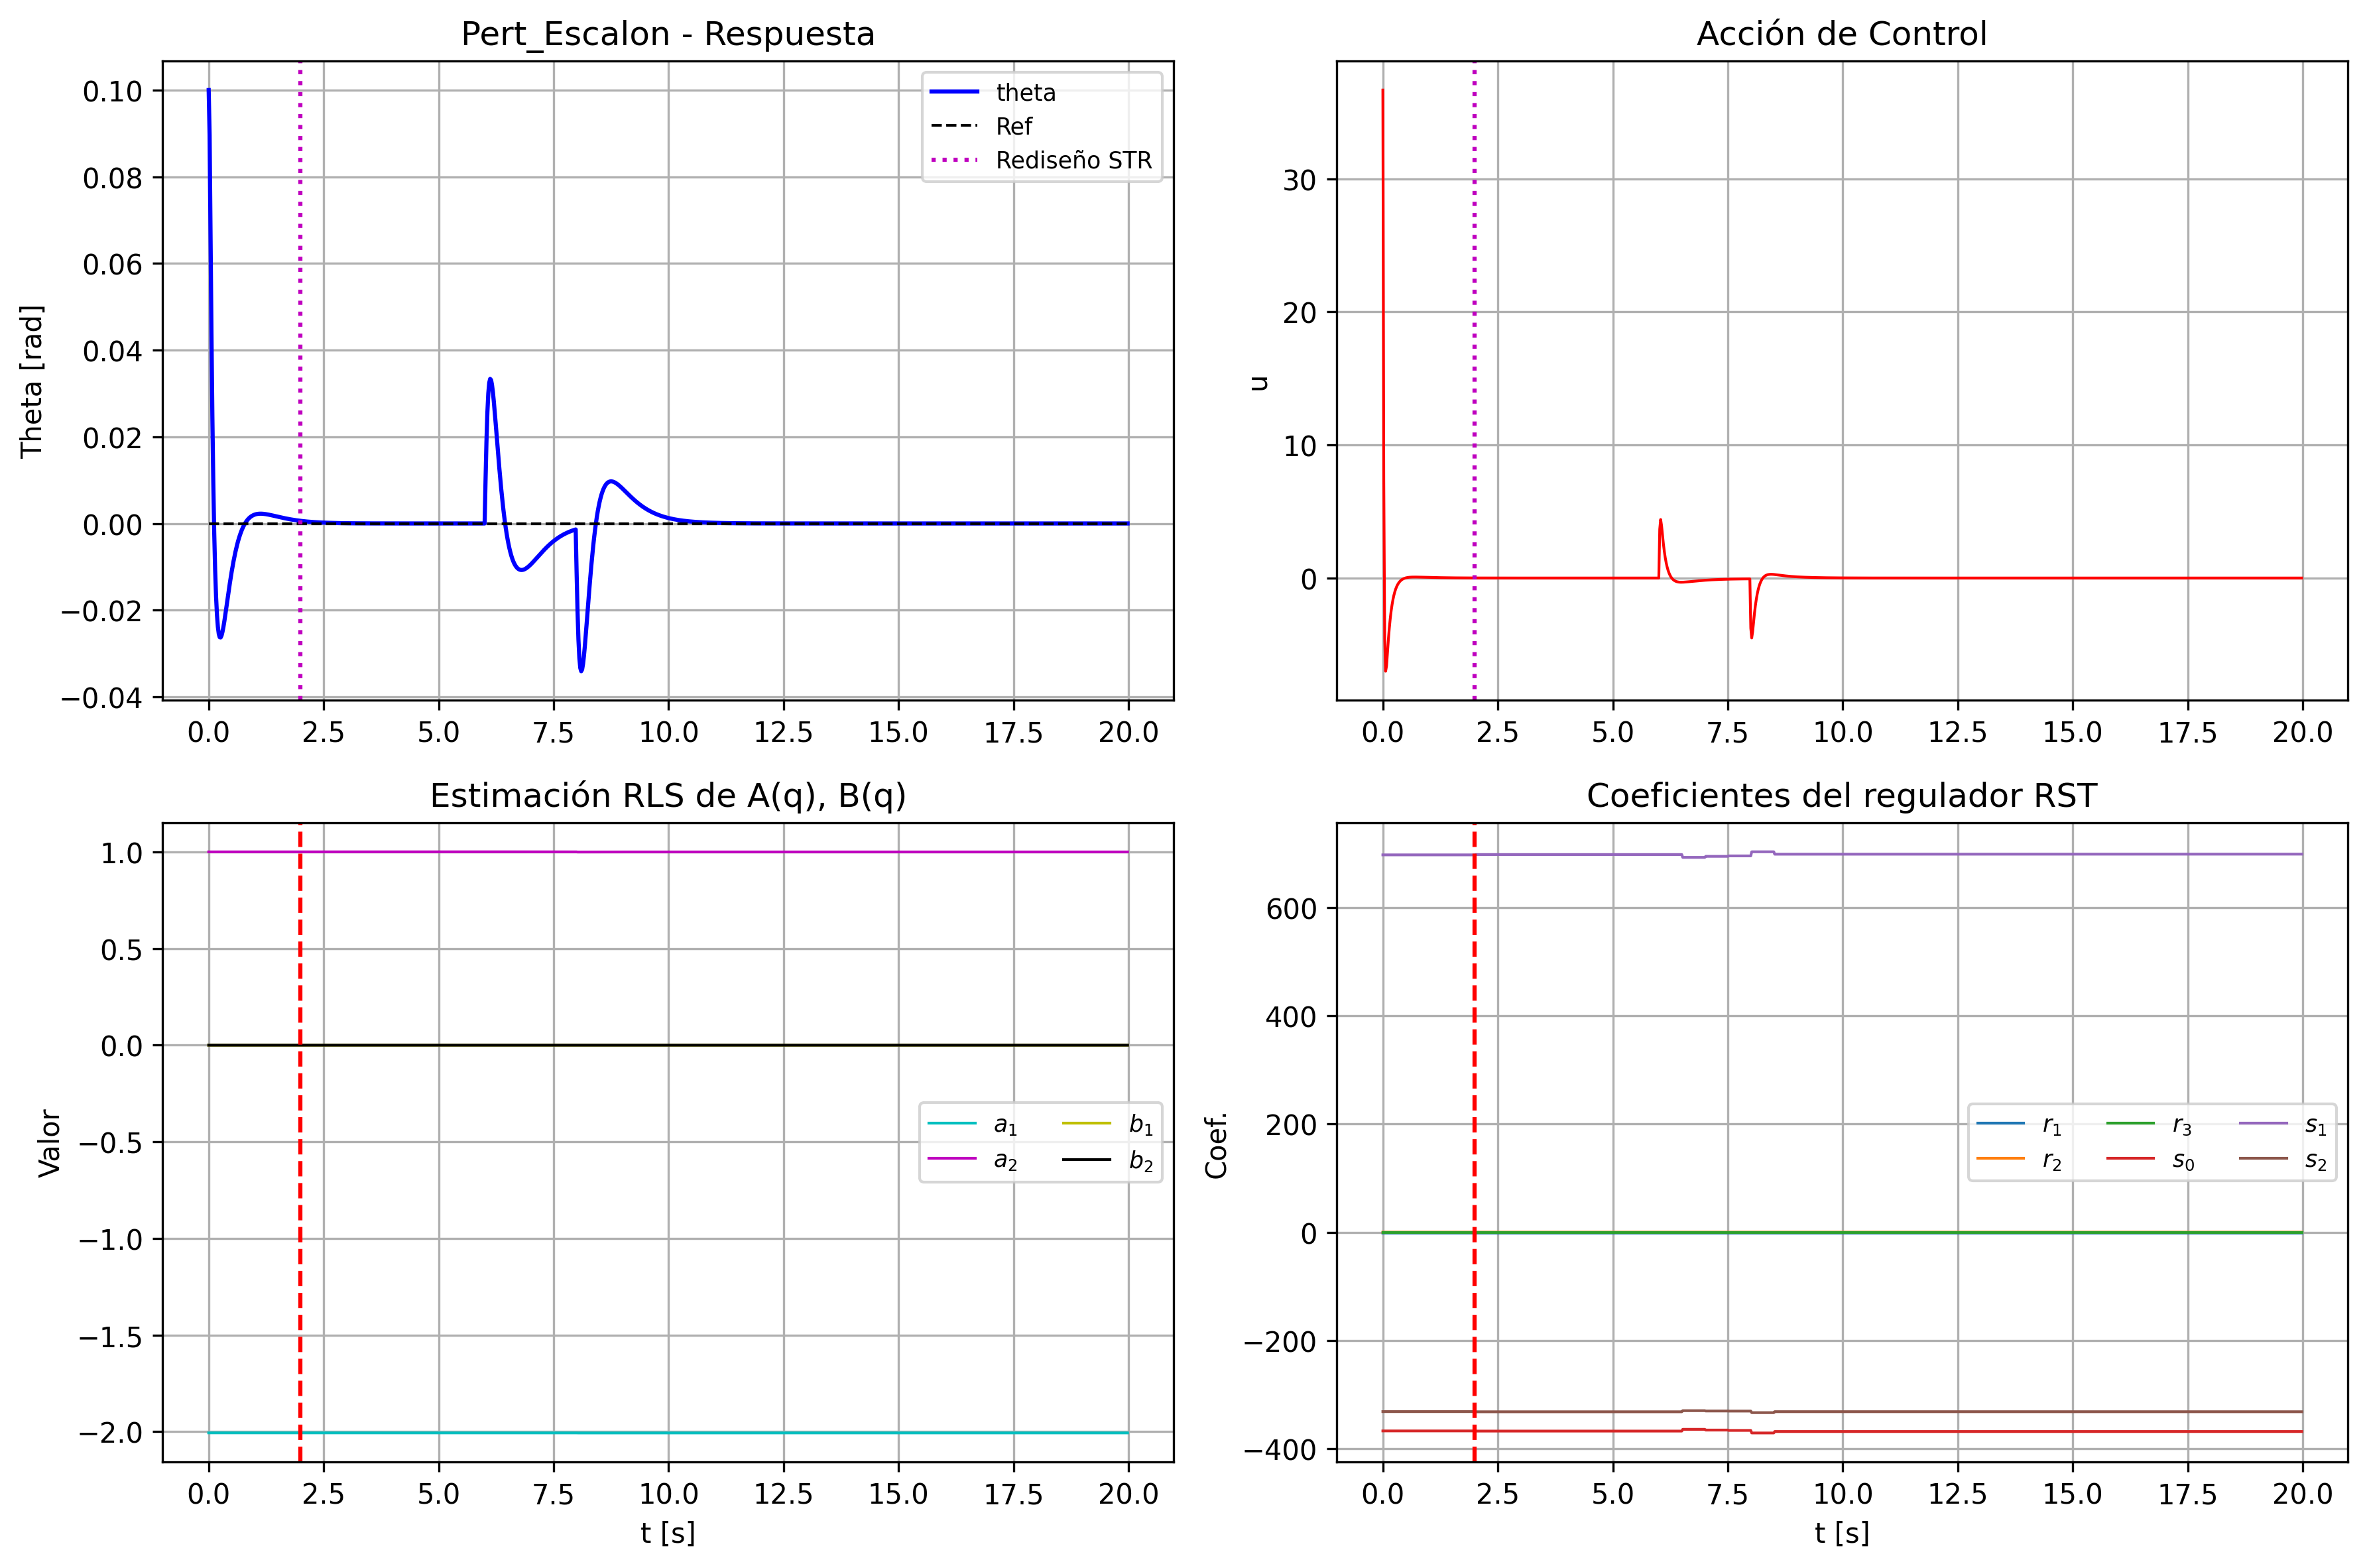
\includegraphics[width=\textwidth]{presentacion_pid_pendulo/imagenes_pid_autotunning/str_Pert_Escalon.png}
  \caption{Perturbación escalón ($t\in[6,8]$)}
\end{subfigure}
\hfill
\begin{subfigure}{0.49\textwidth}
  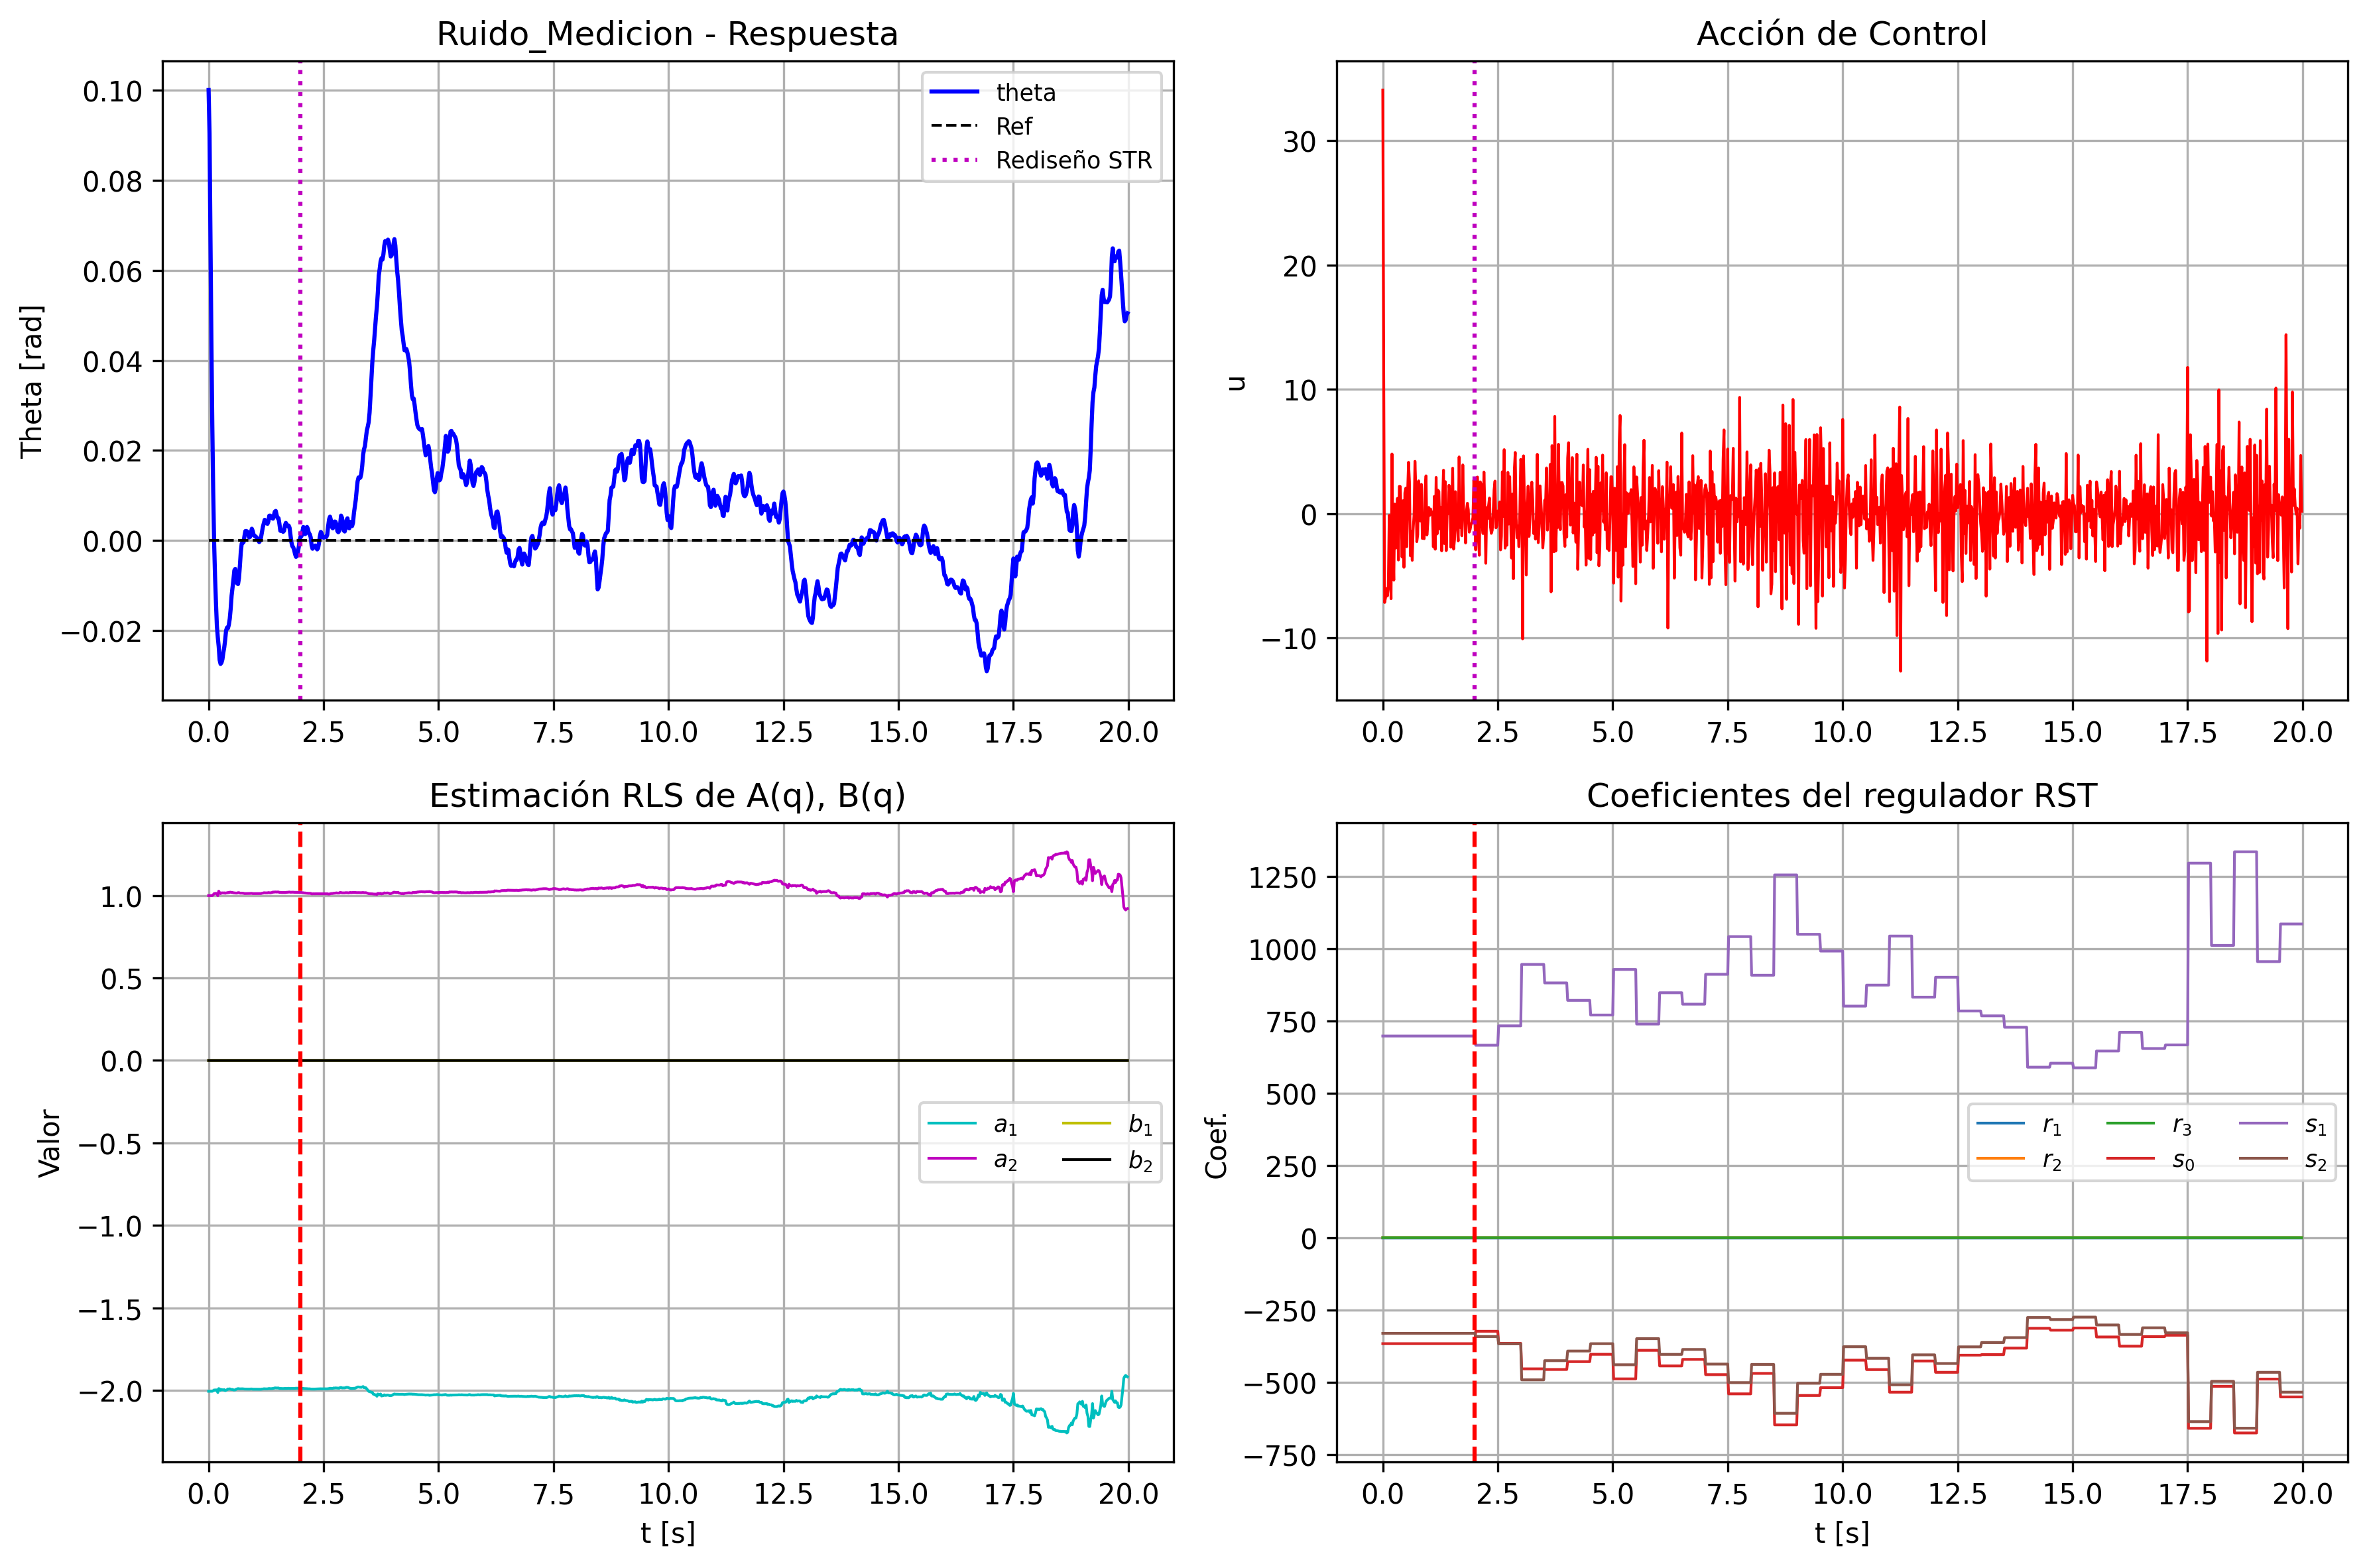
\includegraphics[width=\textwidth]{presentacion_pid_pendulo/imagenes_pid_autotunning/str_Ruido_Medicion.png}
  \caption{Ruido de medición ($\sigma=0{,}005$)}
\end{subfigure}
\caption{Respuesta ($\theta$), acción de control ($u$), estimación RLS de
$A(q),B(q)$ y coeficientes del regulador RST para los cuatro escenarios.}
\label{fig:res}
\end{figure}

\begin{table}[H]
\centering
\caption{Resumen cuantitativo de la validación.}
\begin{tabular}{@{}lccc@{}}
\toprule
Escenario & $|\theta|_{\max}$ [rad] & $|u|_{\max}$ [N] & Estable \\
\midrule
Sin perturbaciones     & 0{,}100 & 36{,}7 & Sí \\
Perturbación sinusoidal & 0{,}100 & 36{,}7 & Sí \\
Perturbación escalón   & 0{,}100 & 36{,}7 & Sí \\
Ruido de medición      & 0{,}100 & 35{,}0 & Sí \\
\bottomrule
\end{tabular}
\end{table}

El integrador $(1-q^{-1})$ en $R$ garantiza error estacionario nulo y rechazo de
la perturbación escalón: el factor $(1-q^{-1})$ cancela el polo en $z=1$ del
escalón, por lo que su efecto permanente sobre la salida es cero.

% ==================================================================
\section{Análisis de estabilidad y convergencia; robustez}
% ==================================================================

El ángulo $\theta$ permanece acotado en los cuatro escenarios, pero un análisis
más fino revela que \textbf{los coeficientes del regulador $R,S,T$ no convergen}
con perturbación sinusoidal ni con ruido de medición. Esta sección lo diagnostica,
lo corrige con una variante \emph{robusta} y valida todo con una suite de tests.

\subsection{Verificación del diseño}

Con el modelo nominal, la solución de la Diofantina reproduce \emph{exactamente}
los polos deseados: las raíces de $A(q)R(q)+B(q)S(q)$ coinciden con $A_{lc}$
($\max|z| = 0{,}9418 < 1$). Los polos elegidos (mapeo $e^{sT_s}$ de $-3,-3,-10$
más dos auxiliares en $0{,}2$) son sensatos: reales, positivos y bien dentro del
círculo unitario. El test \texttt{test\_diophantine\_nominal} verifica esta
igualdad automáticamente.

\subsection{Por qué el regulador no converge (modo básico)}

La ley de control aplicada a la planta \emph{real} usa el regulador diseñado con
el modelo \emph{estimado}. Cuando ese estimado se degrada, el regulador
``persigue'' el ruido. La causa raíz es que el numerador $B$ es diminuto
($b_1{+}b_2 \approx -5{,}9\times10^{-4}$) y aparece en el \emph{denominador} del
diseño ($t_0 = A_{lc}(1)/B(1)$ y la matriz de Sylvester): un error relativo en
$b$ se amplifica enormemente en $R,S,T$. Concretamente:
\begin{itemize}[nosep]
  \item \textbf{Sinusoidal:} la perturbación (inyectada en la salida) hace que el
  RLS reparta mal la ganancia; $b_1$ llega a cambiar de signo, el cero estimado
  salta a $z\approx+1{,}7$ y $s_0$ crece $\sim4\times$ sin estabilizarse.
  \item \textbf{Ruido:} el RLS adapta sobre el ruido (agravado por
  \emph{covariance windup} con $\lambda<1$ y baja excitación); $a_1,a_2$ quedan
  sesgados y $s_0$ fluctúa $\pm20\%$.
\end{itemize}
Aun así el lazo se mantiene estable, pero los polos logrados \emph{sobre la
planta real} se corren hacia el círculo unitario (Tabla~\ref{tab:conv}),
perdiendo margen.

\subsection{Mejoras de robustez}

Se agrega una variante robusta (\texttt{robust=True}), comparable con la básica:
\begin{itemize}[nosep]
  \item \textbf{Regresor consistente} con la salida medida (errores-en-variables).
  \item \textbf{Zona muerta} en el RLS: no se actualiza si $|\varepsilon|$ no
  supera el error de ecuación esperado ($\sim\sigma\lVert[1,a_1,a_2]\rVert$),
  evitando adaptar sobre ruido/perturbación puros.
  \item \textbf{Anti \emph{windup} de covarianza}: se acota $\mathrm{tr}(P)$.
  \item \textbf{Gate de rediseño} validado contra el \emph{prior nominal
  confiable} (no contra la estimación ruidosa): se acepta un candidato solo si
  $b_1{+}b_2$ conserva signo y magnitud, $|t_0|$ y $\lVert S\rVert$ son
  razonables y el lazo cerrado resultante es estable. Además solo se rediseña
  ante cambios significativos de $\hat\theta$ (congelamiento).
\end{itemize}

\begin{lstlisting}[caption={Gate de aceptación del regulador candidato (robusto).}]
def candidato_valido(R, S, t0, theta_hat, s_norm_max, cfg, plant_ref):
    b1, b2 = theta_hat[2], theta_hat[3]
    if (b1 + b2) >= 0 or abs(b1 + b2) < cfg["b_min"]:   # signo/magnitud de b
        return False
    if abs(t0) > cfg["t0_max"] or np.linalg.norm(S) > s_norm_max:
        return False
    poles = closed_loop_poles(plant_ref, R, S)          # estabilidad vs prior
    return np.max(np.abs(poles)) < 1.0 - cfg["pole_margin"]
\end{lstlisting}

\subsection{Resultados comparativos}

La variante robusta hace converger $R,S,T$ y recupera exactamente los polos de
diseño ($\max|z| = 0{,}9418$) en los cuatro escenarios, mientras la básica deriva
(Tabla~\ref{tab:conv}, Figuras~\ref{fig:conv} y \ref{fig:cmp}).

\begin{table}[H]
\centering
\caption{Estabilidad (máx.\ módulo de polo de LC sobre la planta real con el
regulador final) y convergencia (desvío de $s_0$ en la ventana final).}
\label{tab:conv}
\begin{tabular}{@{}lcccc@{}}
\toprule
& \multicolumn{2}{c}{Básico} & \multicolumn{2}{c}{Robusto} \\
\cmidrule(lr){2-3}\cmidrule(lr){4-5}
Escenario & $\max|z|$ & std$(s_0)$ & $\max|z|$ & std$(s_0)$ \\
\midrule
Sin perturbaciones      & 0{,}942 & $\approx 0$ & 0{,}942 & $0$ \\
Perturbación sinusoidal & 0{,}989 & $190$       & 0{,}942 & $0$ \\
Perturbación escalón    & 0{,}957 & $\approx 0$ & 0{,}942 & $0$ \\
Ruido de medición       & 0{,}995 & $126$       & 0{,}942 & $0$ \\
\bottomrule
\end{tabular}
\end{table}

\begin{figure}[H]
\centering
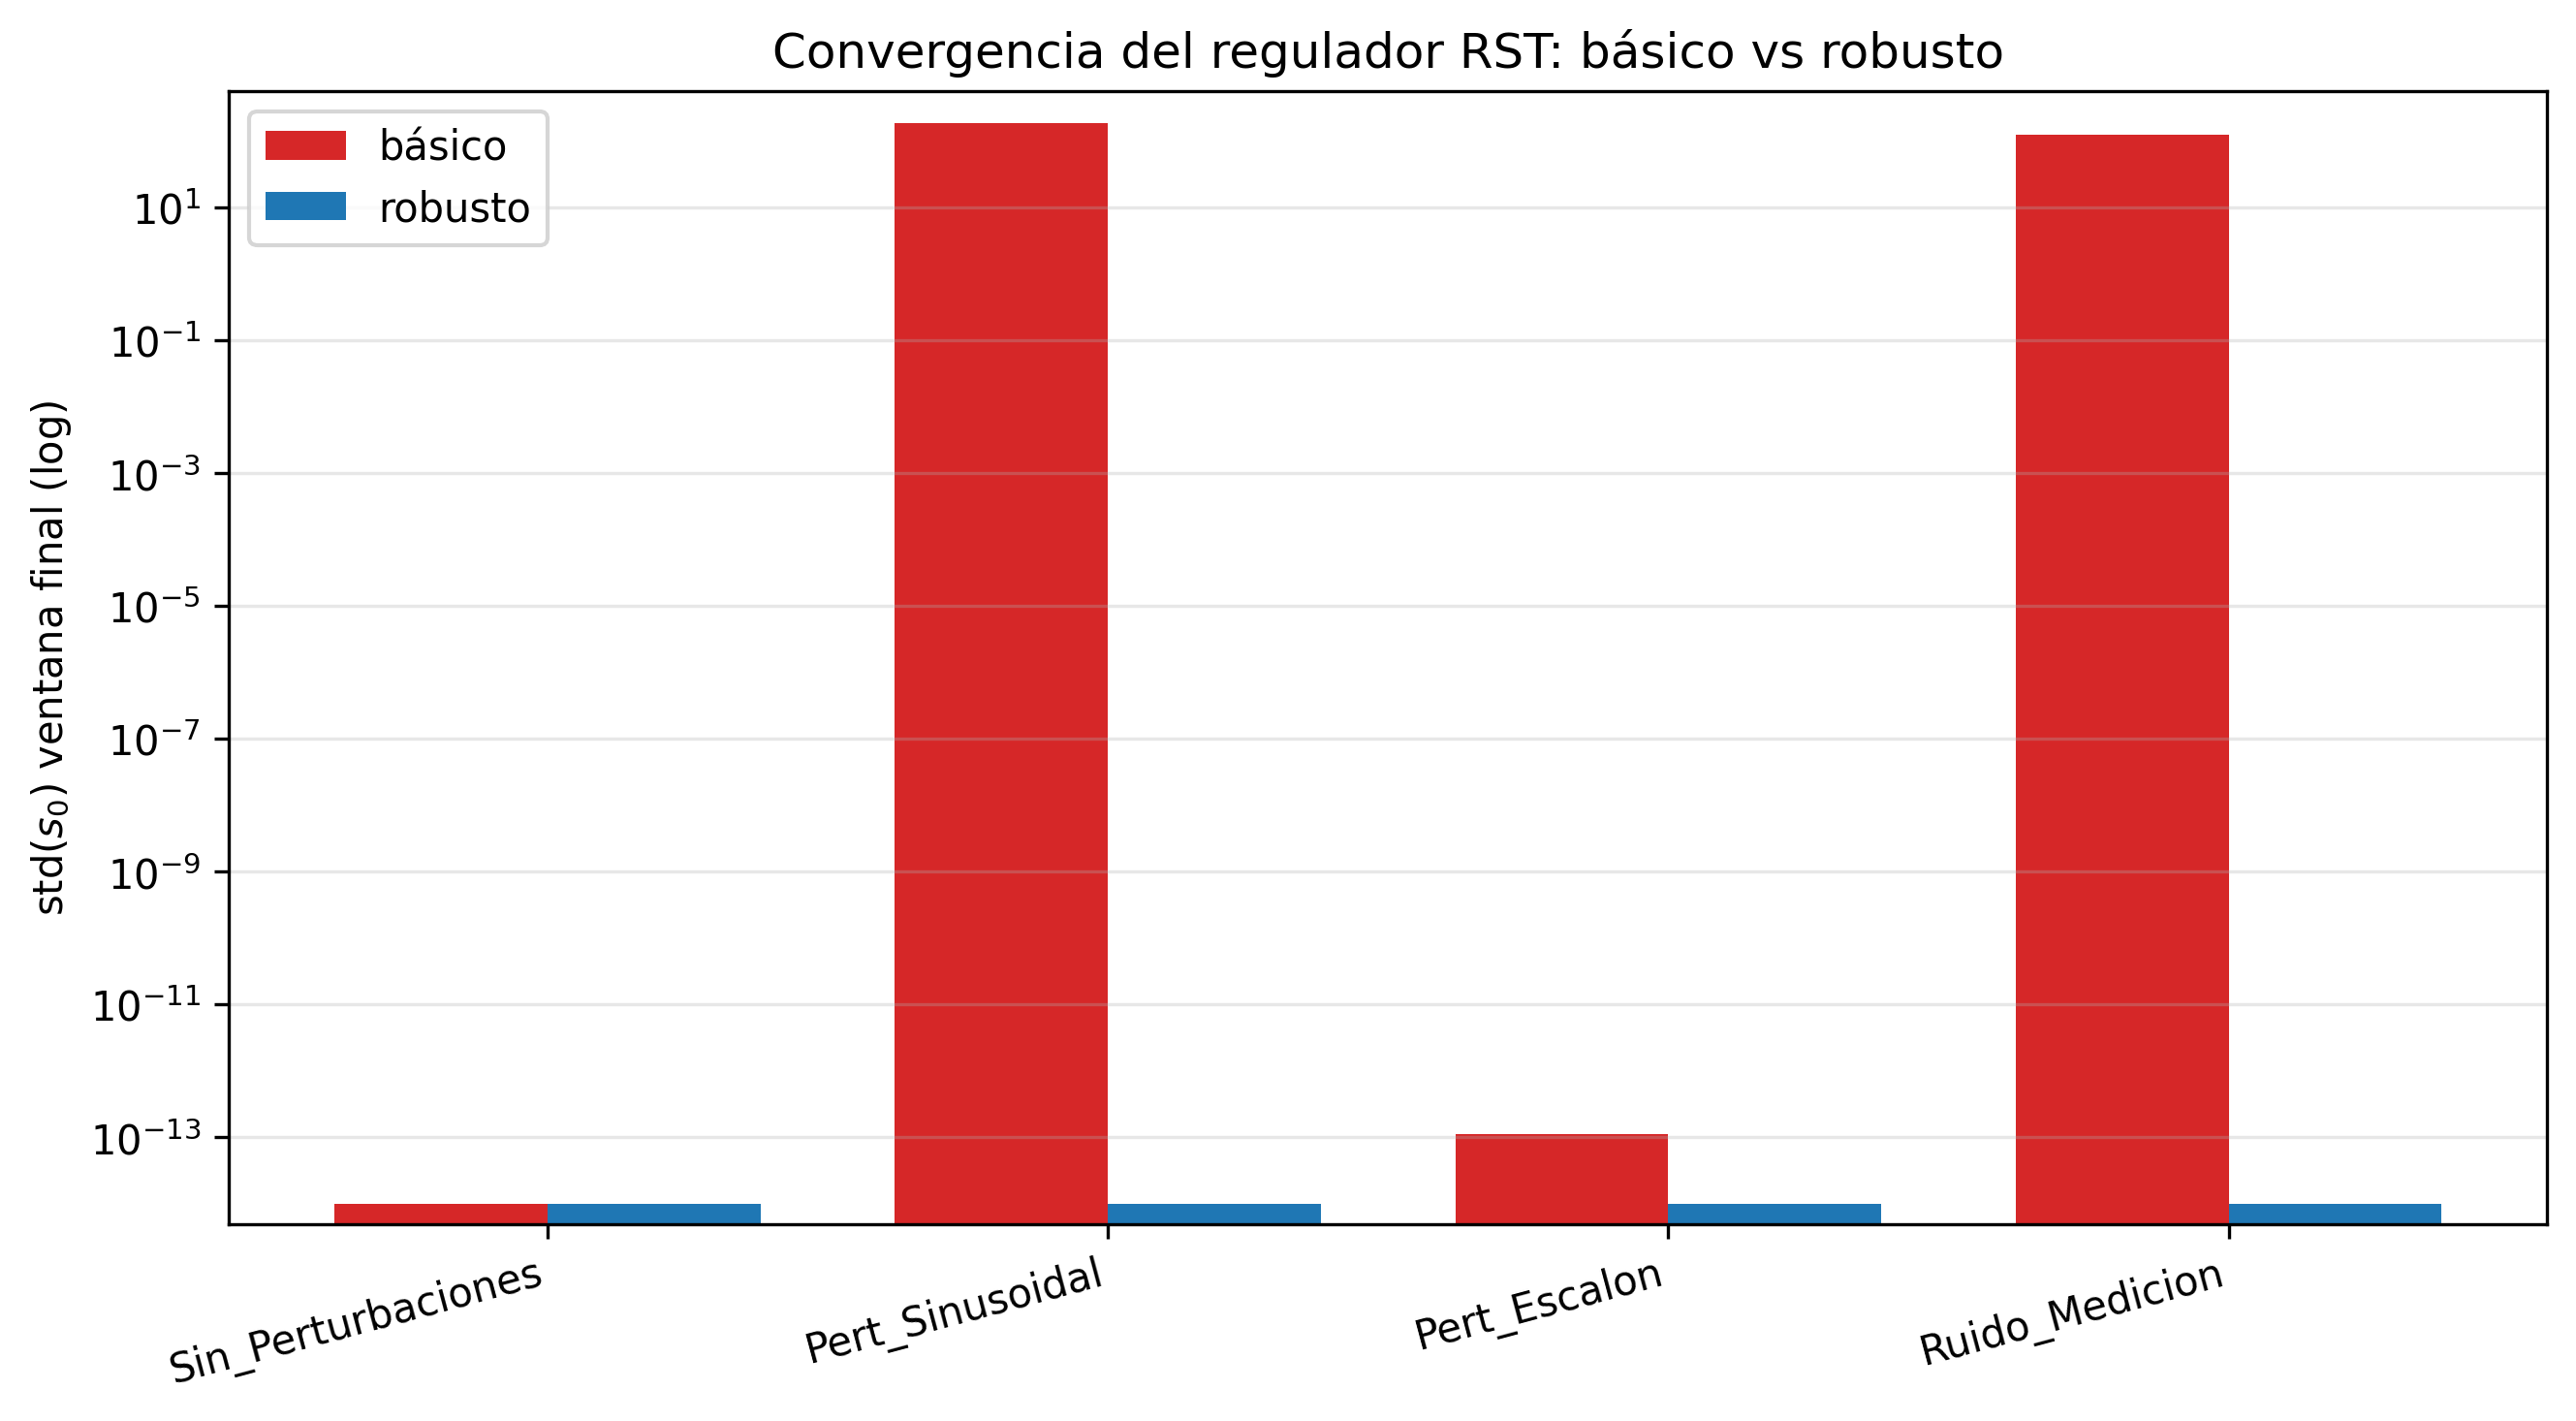
\includegraphics[width=0.8\textwidth]{presentacion_pid_pendulo/imagenes_pid_autotunning/str_convergencia.png}
\caption{Desvío estándar de $s_0$ en la ventana final (escala log). El modo
robusto (azul, prácticamente nulo) converge en todos los escenarios; el básico
(rojo) no converge con perturbación sinusoidal ni con ruido.}
\label{fig:conv}
\end{figure}

\begin{figure}[H]
\centering
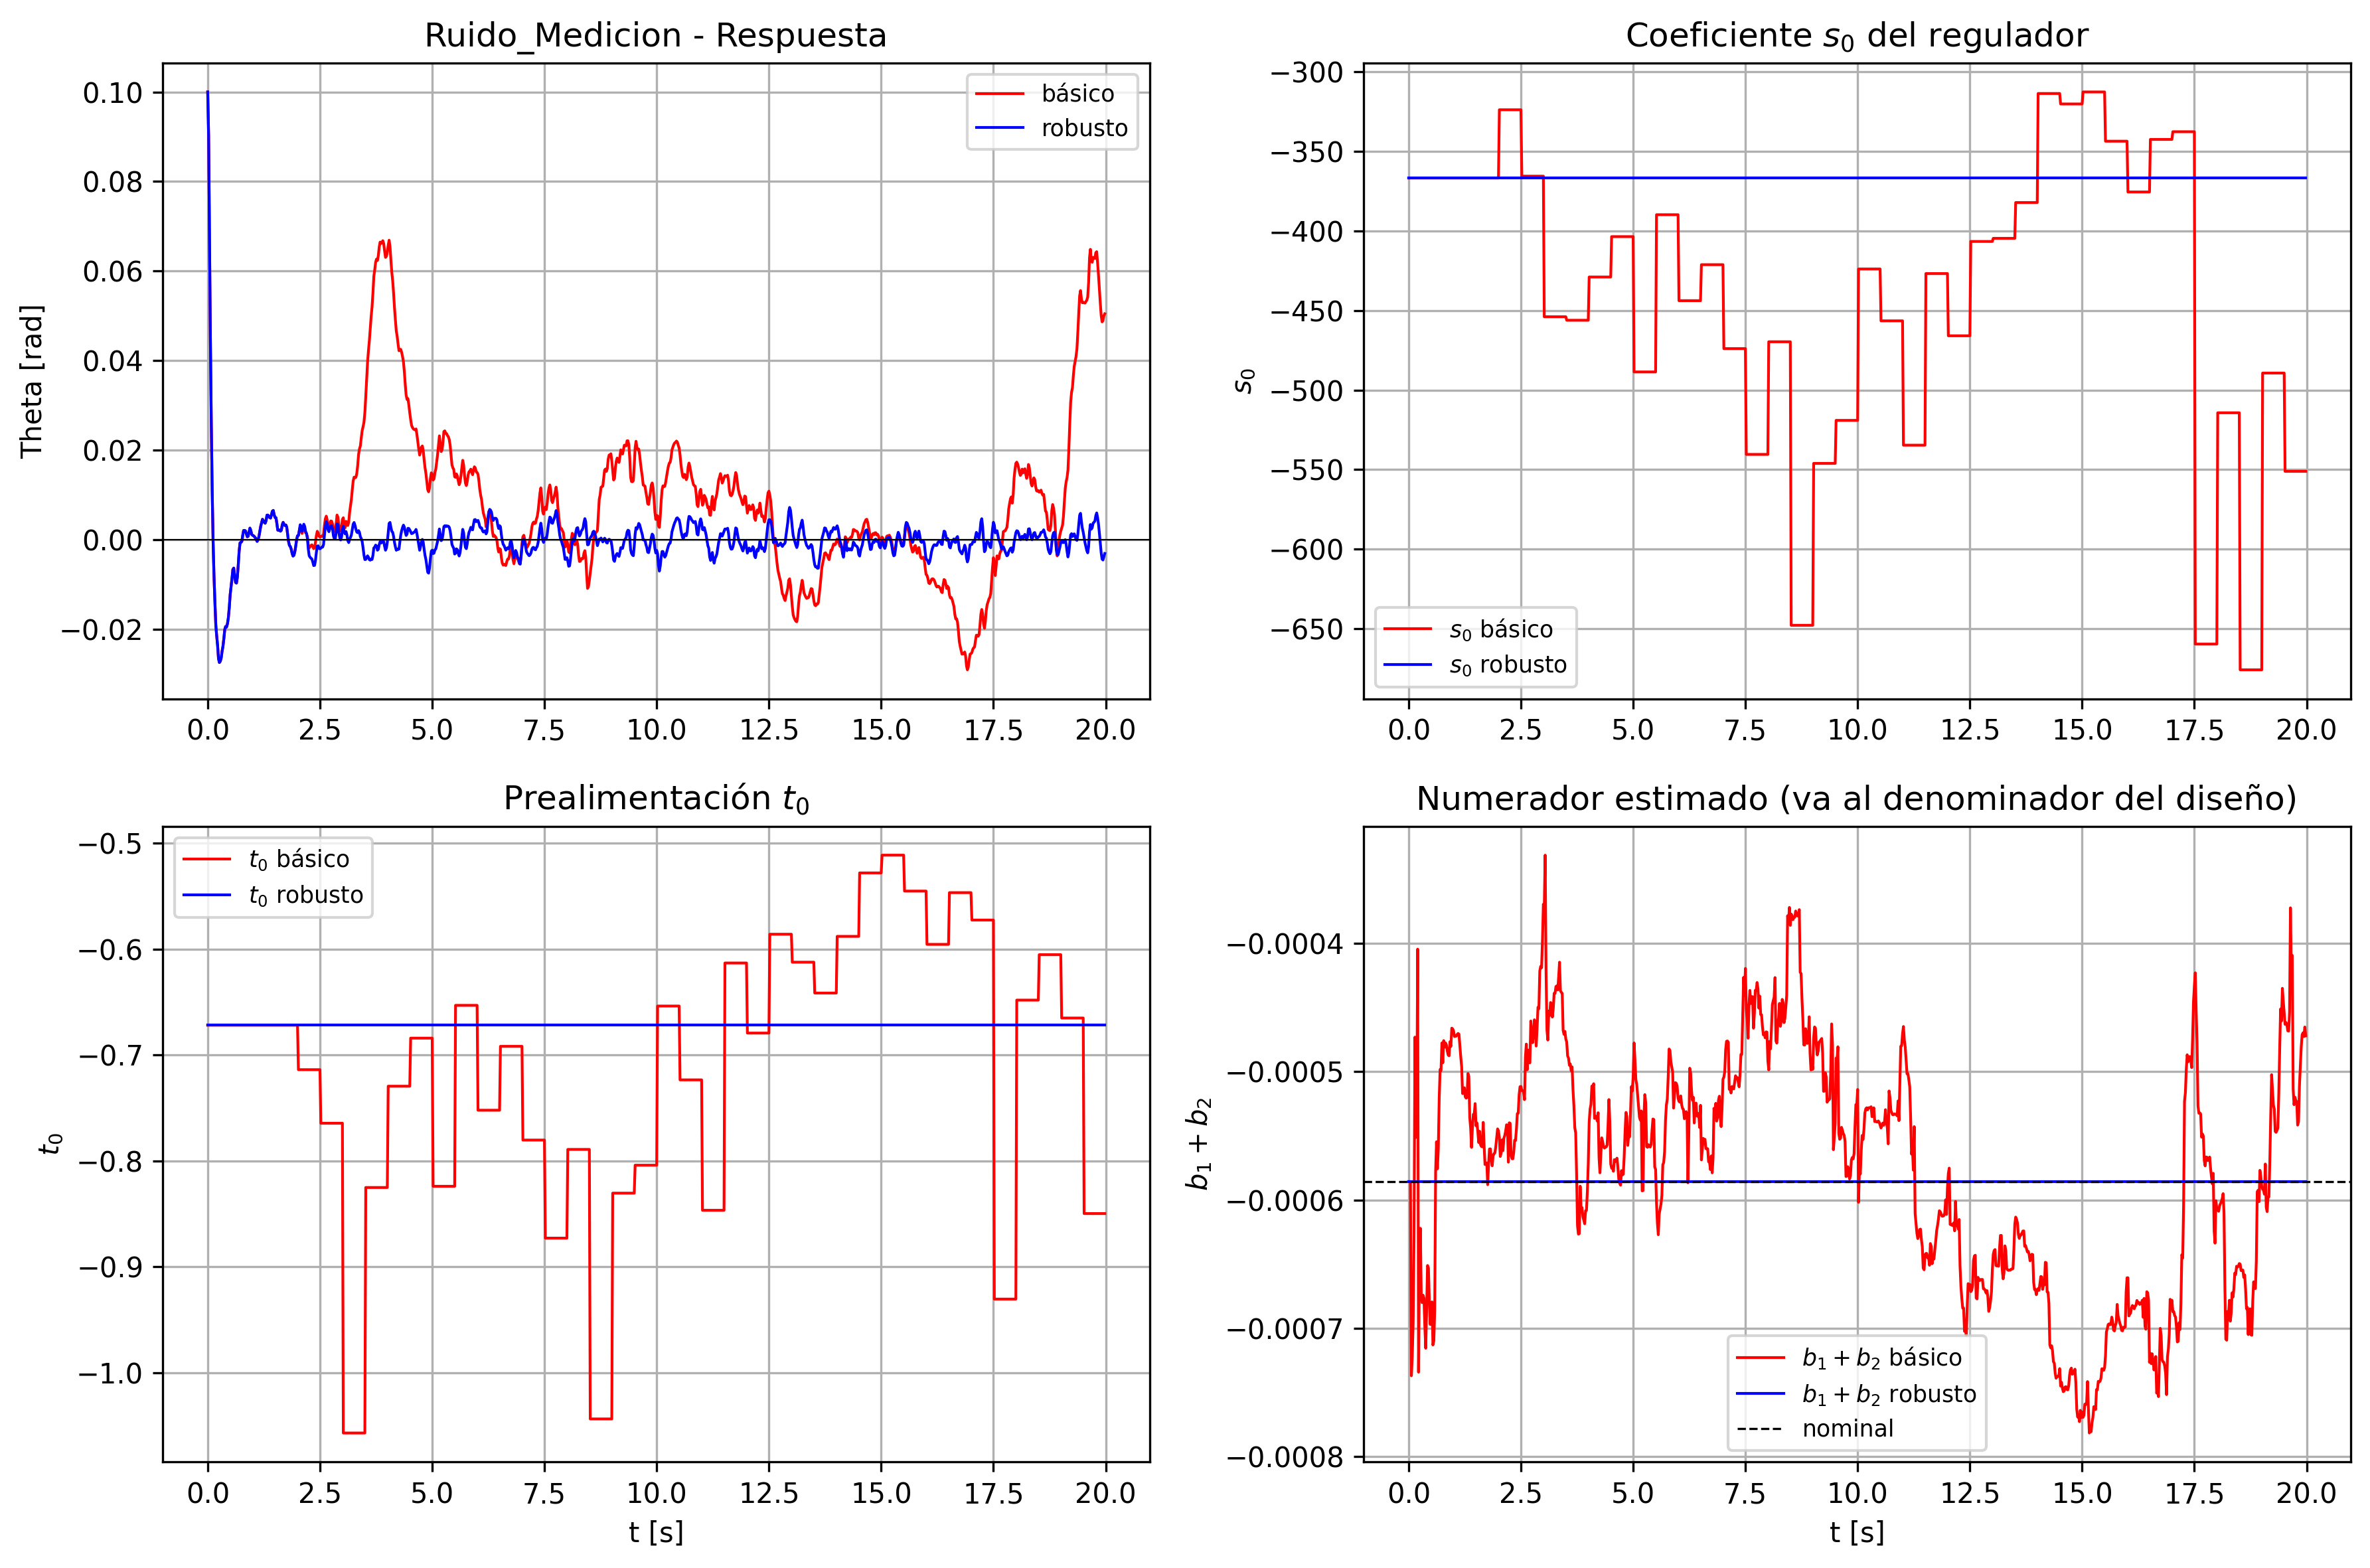
\includegraphics[width=0.9\textwidth]{presentacion_pid_pendulo/imagenes_pid_autotunning/str_cmp_Ruido_Medicion.png}
\caption{Ruido de medición: básico (rojo) vs robusto (azul). El regulador básico
persigue el ruido ($s_0$, $t_0$ y $b_1{+}b_2$ oscilan); el robusto se estabiliza
en el diseño nominal y además regula mejor a $\theta$.}
\label{fig:cmp}
\end{figure}

\subsection{Suite de validación}

El archivo \texttt{test\_str\_pendulo.py} automatiza la validación (todos los
tests pasan):
\begin{itemize}[nosep]
  \item \texttt{test\_diophantine\_nominal}: el diseño nominal reproduce $A_{lc}$.
  \item \texttt{test\_estabilidad\_lazo}: $\max|z|<1$ en los 4 escenarios y ambos
  modos.
  \item \texttt{test\_theta\_acotado}: $|\theta|\le 0{,}12$ en todos los casos.
  \item \texttt{test\_convergencia\_RST\_robusto} y
  \texttt{test\_robusto\_mejora\_convergencia}: $R,S,T$ convergen en robusto y
  mejoran respecto del básico en sinusoidal/ruido.
  \item \texttt{test\_convergencia\_RLS\_robusto}: $\hat\theta$ cercano al modelo
  real.
\end{itemize}

% ==================================================================
\section{Discusión}
% ==================================================================

\begin{itemize}[nosep]
  \item \textbf{Persistencia de excitación.} Al ser una tarea de regulación
  ($\theta \to 0$), una vez estabilizado el sistema la excitación se desvanece.
  Por eso el RLS arranca desde el \emph{prior} nominal y se congela la
  actualización con baja excitación: así el \emph{certainty equivalence} se
  mantiene bien condicionado y estable. Iniciar el estimador desde un prior
  neutro provocó, en pruebas, deriva de parámetros y divergencia, en línea con
  las advertencias de \texttt{ICA\_STR.pdf}.
  \item \textbf{No cancelación de ceros.} El cero en $z\approx-1$ es no de fase
  mínima; cancelarlo produciría \emph{ringing}. La colocación de polos sin
  cancelación evita este problema.
  \item \textbf{Comparación con el enfoque previo.} El STR discreto obtiene el
  regulador directamente en $z$ resolviendo la Diofantina, eliminando la
  conversión a continuo por Tustin y la colocación de polos en $s$. El
  resultado es equivalente pero conceptualmente más directo y consistente con la
  implementación digital.
\end{itemize}

% ==================================================================
\section{Conclusiones}
% ==================================================================

Se implementó y validó un Self-Tuning Regulator adaptativo indirecto,
enteramente en tiempo discreto, que estabiliza el péndulo invertido inestable.
El método combina estimación RLS on-line, resolución de la ecuación Diofantina
por matriz de Sylvester (con integrador y sin cancelar el cero no de fase
mínima) y la ley de control RST. La validación muestra estabilización desde la
condición inicial, convergencia de los parámetros estimados a los valores reales
y rechazo de perturbaciones de carga y ruido de medición, cumpliendo con la
definición de \emph{self-tuning}: el regulador converge al que se hubiese
diseñado conociendo la planta.

Como material adicional se generan animaciones (\texttt{.mp4}) de cada escenario
en \texttt{saved\_runs\_pid\_autotunning/}.

% ==================================================================
\begin{thebibliography}{9}
\bibitem{str} P. González, \emph{Identificación y Control Adaptativo: STR},
FIUBA, 2025 (\texttt{ICA\_STR.pdf}).
\end{thebibliography}

\end{document}
